%%%%%%%%%%%%%%%%%%%%%%%%%%%%%%%%%%%%%%%%%%%%%%%%%%%%%%%%%%%%%%%%%%%%%%%%
%    INSTITUTE OF PHYSICS PUBLISHING                                   %
%                                                                      %
%   `Preparing an article for publication in an Institute of Physics   %
%    Publishing journal using LaTeX'                                   %
%                                                                      %
%    LaTeX source code `ioplau2e.tex' used to generate `author         %
%    guidelines', the documentation explaining and demonstrating use   %
%    of the Institute of Physics Publishing LaTeX preprint files       %
%    `iopart.cls, iopart12.clo and iopart10.clo'.                      %
%                                                                      %
%    `ioplau2e.tex' itself uses LaTeX with `iopart.cls'                %
%                                                                      %
%%%%%%%%%%%%%%%%%%%%%%%%%%%%%%%%%%
%
%
% First we have a character check
%
% ! exclamation mark    " double quote  
% # hash                ` opening quote (grave)
% & ampersand           ' closing quote (acute)
% $ dollar              % percent       
% ( open parenthesis    ) close paren.  
% - hyphen              = equals sign
% | vertical bar        ~ tilde         
% @ at sign             _ underscore
% { open curly brace    } close curly   
% [ open square         ] close square bracket
% + plus sign           ; semi-colon    
% * asterisk            : colon
% < open angle bracket  > close angle   
% , comma               . full stop
% ? question mark       / forward slash 
% \ backslash           ^ circumflex
%
% ABCDEFGHIJKLMNOPQRSTUVWXYZ 
% abcdefghijklmnopqrstuvwxyz 
% 1234567890
%
%%%%%%%%%%%%%%%%%%%%%%%%%%%%%%%%%%%%%%%%%%%%%%%%%%%%%%%%%%%%%%%%%%%
%

\documentclass[12pt]{iopart}
\usepackage[dvipsnames]{xcolor}
\usepackage{graphicx}
\usepackage[sorting=none]{biblatex} %Imports biblatex package
\addbibresource{references.bib} %Import the bibliography file
\newcommand{\gguide}{{\it Preparing graphics for IOP Publishing journals}}
%Uncomment next line if AMS fonts required
%\usepackage{iopams}  
\graphicspath{{Figures/}}

\begin{document}

\title{Using Machine Learning to predict the behavior of moderate pressure capacitively coupled plasmas}
%JMP is a specific bit of software that is used to do designed experiments - and similar studies. That is NOT new. What is important here is the ML bit.
\author{Shadhin Hussain,$^{ a}$ David J. Lary,$^{ a}$ Ken Hara,$^{b}$ Kallol Bera,$^{c}$ Shahid Rauf,$^{c}$  Matthew Goeckner$^a$}

\address{$^a$Department of Physics, University of Texas at Dallas, Richardson TX, 75080 \\
$^b$Aeronautics and Astronautics, Stanford University,  Stanford CA, 94305 \\
$^c$Applied Materials Corp, Santa Clara, CA 95054}
\ead{Shadhin.Hussain@utdallas.edu, david.lary@utdallas.edu, \\ kenhara@stanford.edu, Kallol\_Bera@amat.com, Shahid\_Rauf@amat.com, goeckner@utdallas.edu}
\vspace{10pt}
\begin{indented}
\item[]February 2023
\end{indented}

\begin{abstract}
\textcolor{red}{One two three... need to write this.}
\end{abstract}

%
% Uncomment for keywords
%\vspace{2pc}
%\noindent{\it Keywords}: XXXXXX, YYYYYYYY, ZZZZZZZZZ
%
% Uncomment for Submitted to journal title message
%\submitto{\JPA}
%
% Uncomment if a separate title page is required
%\maketitle
% 
% For two-column output uncomment the next line and choose [10pt] rather than [12pt] in the \documentclass declaration
%\ioptwocol
%



\section{Introduction}

\textbf{ Introduction needs to be rewritten with more emphasis on ML }\\

Machine learning allows us to \textit{learn by example}, and to \textit{give our data a voice}. It is especially useful for applications for which we do \textit{not} has a complete theory but are of interest to us. Machine learning is an automated implementation of the scientific method \cite{Domingos:2015}, following the same process of generating, testing and discarding or refining hypotheses. While a scientist or engineer may spend his entire career coming up with and testing a few hundred hypotheses, a machine-learning system can do the same in a fraction of a second. Machine learning provides an objective set of tools for automating discovery. It is therefore not surprising that machine learning is currently revolutionizing many areas of science, technology, business and medicine \cite{Lary:2016}.

Machine Learning (ML) holds the potential to expand our understanding of laboratory plasmas operating under conditions that are largely unexplored.[NEEDS REF]  Laboratory plasmas are complex environments that are influenced by many external `control parameters'. These control parameters include: external power (power deposition method, power level, supplied power frequency); neutral gas (species, pressure, flow rate); chamber geometry/materials.  Understanding fundamental physical phenomena such as collision, diffusion, particle and energy balance, and gas chemistry is essential to comprehending the processes that govern plasma dynamics at different conditions.  Under some conditions, it is possible to deploy a large suite of diagnostics and via those results develop effective models of the plasma system.  Under other conditions, such as intermediate or high pressures, traditional diagnostics (Langmuir probes, etc) will not function correctly and detailed models of the plasmas are harder to develop.  Early results with ML already show promise in bridging this gap. [NEEDS REF]

Capacitively coupled plasmas (CCPs) are one of the most commonly used laboratory plasmas, due to their wide use in the semiconductor industry.  CCPs are commonly classified by their operating pressure and the resulting ``heating mode.'' [NEEDS REF] A low-pressure discharge is typically considered to be within the range of tens of µTorr up to tens of mTorr, while the moderate/intermediate pressure regime spans from 1-100 Torr.[NEEDS REF] These two pressure regimes differ significantly in terms of breakdown, heating, and maintaining the discharge.[NEEDS REF] 

Although the general pressure dependence of CCPs is known, studies of these systems in the intermediate pressure regime are limited.  This is in part because `traditional' diagnostic tools, such as Langmuir Probes, do not work at these intermediate pressures.[NEEDS REF]  None-the-less, such intermediate pressure CCP systems are widely utilized in industrial applications, including carbon nanotube and diamond-like carbon deposition processes, flat panel display and solar panel fabrication industries, as well as an active medium for CO2 lasers. However, despite their widespread use, a lack of understanding of radio frequency (RF) CCP discharges in these pressure ranges has resulted in most designs being based on empirical studies.

Modeling and forecasting the dynamics of complex systems such as intermediate pressure CCP systems remains a challenge due to the interactions of physical and chemical processes across multiple scales. Observational data, including multi-fidelity data from sensors, can provide valuable insights, but integrating it into existing models is difficult. On the other hand, Machine Learning (ML) approaches, particularly deep learning, can extract features from massive amounts of data, but may lack interpretability and physical consistency.

In this article, we will examine the use of ML to predict trends in moderate pressure CCPs.  Here, we make use of a  Design of Experiment (DOE)  organized experimental study of the current-voltage (I-V) signal in the deposited power. We will explore the efficacy of various ML models on the resultant I-V data sets in predicting I-V data under other conditions. We will show results and compare the prediction accuracy of different ML models including supervised regression as well as supervised classification approaches, as well as of least square fitting using a common DOE software tool (JMP).

In section \ref{Sect:ExpSetup} we will describe the experimental system and related diagnostic tools.  This will include a review of how the measured data is analyzed to arrive at our database.  In section \ref{Sect:Database} we will present the resultant data that will be used in the our ML study. In section 
\ref{Sect:RegressionAnalysis} we will deploy four common ML regression analysis models to examine our experimental data.  In section \ref{Sect:Classification} we will explore ML classification models with our experimental data. Finally we provide our conclusions in section \ref{Sect:Conclusions}.

\section{Experimental setup}\label{Sect:ExpSetup}
The experiments used for these studies were conducted in the modified Gaseous Electronics Conference (mGEC) system \cite{goeckner2004modified,hernandez2020electron,hernandez2021optical,press2019sub}. The design of the modified Gaseous Electronics Conference (mGEC) chamber, with an inductively coupled source, has been discussed in detail by Goeckner \textit{et al}. \cite{goeckner2004modified}. The mGEC with a CCP source is discussed in detail in works by Hernandez \textit{et al.} and Press \textit{et al}. \cite{hernandez2020electron,hernandez2021optical,press2019sub} A general sketch of the system is shown in Figure \ref{Fig:mGEC}. The powered electrode facing the plasma is made of aluminum and has a diameter of 11.4 cm while the diameter of the grounded electrode is 15 cm. The gap between the powered electrode and the grounded electrode is adjustable anywhere between 2 cm and 12.5 cm. While internal walls, which would control the effective diameter of the chamber are available for the mGEC, there were not used in these studies. An rf signal generator (Keysight 33600) was used to produce a 13.56 MHz signal which was then passed to an amplifier (ENI A-300) to create the input power.  Baseline measurements of supplied and reflected power were made using a wattmeter (Bird: Model 43).  From there, the power was sent through an L-type match network and on to the powered electrode. The matching network consists of two variable capacitors which can be tuned to match the impedance of the source to that of the load, and thereby minimize the measured reflected power observed in the wattmeter. The load consists of the plasma along with a DC self-bias measurement circuit, current and voltage (I-V) probes, the powered electrode, the 50-ohm transmission line between them, and the grounded chamber, including a grounded electrode/chuck.

\begin{figure}[ht!]
\begin{center}
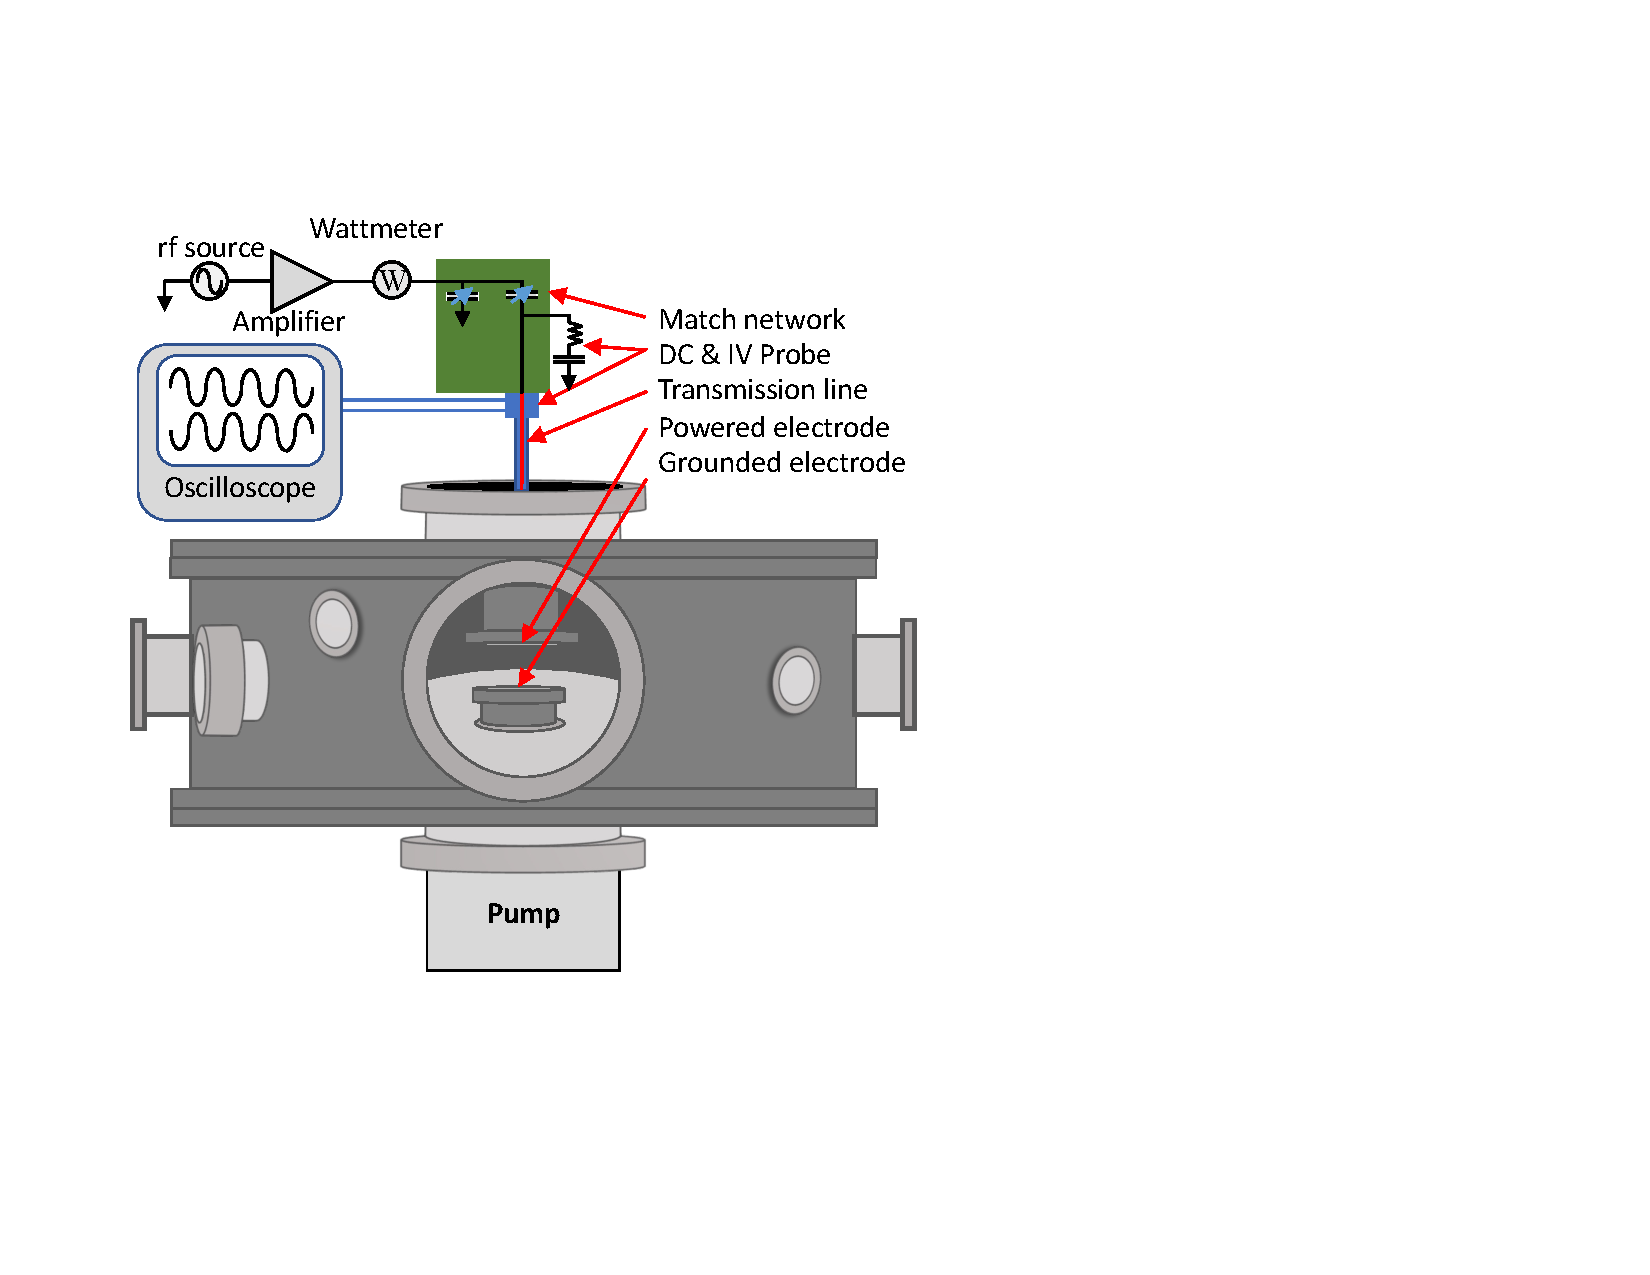
\includegraphics[width=.89\textwidth]{mGEC.pdf}
	\caption{A sketch of the modified Gaseous Electronics Conference (mGEC) reference cell\cite{goeckner2004modified}.  \textbf{Does this need to be edited for copyright rules?}}
	\label{Fig:mGEC}
\end{center}
\end{figure}

The primary diagnostics used in this study include the DC self-bias, rf current and voltage measurements.  All were measured on the 50-ohm transmission line between the match network and the powered electrode as shown in Figure \ref{Fig:mGEC}. As shown in Figure \ref{Fig:mGEC_Circuit}, the DC self-bias measurement system consisted of a series 84 $\mu$ H choke followed by a capacitor to ground, across which the bias was measured.  The current probe was a Rogowski coil (Pearson electronics 2877) while the voltage probe was built by capacitively coupling to the powered lead of the transmission line through a piece of Teflon.  An identical Rogowski coil was also used measure the current through the grounded electrode. A high-speed oscilloscope (Teledyne Lecroy HDO 6104B) with a vertical resolution of 12 bits and a sampling rate of ${10}^{10}$ samples per second was used to acquire all of the RF I-V data, including the relative phase, $\nu$, between the two signals. In order to make the voltage probe diagnostic more sensitive to the relatively small, higher frequency harmonics generated in the plasma sheath, it was connected to the 50-ohm input of the oscilloscope.  In order to distinguish the fundamental and the higher harmonics within the various waveforms, a fast Fourier transform (FFT) analysis was performed on the gathered I-V data.  As a result of this analysis, we were able to determine the I-V amplitudes and relative phases between the current and voltage for the first, second and third harmonics of the applied rf signal.  The full list of all parameters is given in Table \ref{tab:Measured_parameters}.   Such an analysis is essential for calculating the power and impedance characteristics of the sheath as well as the bulk of the plasma.

\begin{figure}[ht!]
\begin{center}
\includegraphics[width=.99\textwidth]{mGEC_Circuit.pdf}
	\caption{Circuit elements of the I-V measurement experiment. Measured parasitic impedances at $Z_1$, $Z_2$,$Z_{g1}$, and $Z_{g2}$ are given in Table \ref{tab:Measured_impedance}. \textbf{Does this need to be edited for copyright rules?}} 
	\label{Fig:mGEC_Circuit}
\end{center}
\end{figure}

\begin{table}[]
    \centering
    \begin{tabular}{|c|c|c|c|c|}
        \hline
        Frequency (MHz) & $Z_1 (\Omega)$ & $Z_2 (\Omega)$ & $Z_{g1} (\Omega)$ & $Z_{g2} (\Omega)$ \\
        \hline
        13.56 & 28.97i & 4.96-113.87i & 1.1+11.95i & -71.79i\\
        27.12 & 0.12+7.6i & 2.39-18.68i & 1.1+23.91i & -35.89i \\
        40.68 & 11.48+81.83i & 2.52+35.96i & 1.1+35.86i & -23.93i \\
        \hline
    \end{tabular}
    \caption{Measured parasitic impedances $Z_1$, $Z_2$, $Z_{g1}$, and $Z_{g2}$.  These values were used to determine the currents and voltages at the electrode faces from the measured values. }
    \label{tab:Measured_impedance}
\end{table}

\begin{table}[]
    \centering
%    \begin{tabular}{|c|c|c|}
\begin{tabular}{|p{1cm}|p{2cm}|p{12.5cm}|}
        \hline
        & Variable & Description\\ 
        \hline
       1 & $V_{DC}$ & DC self-bias\\
       2 & $V_{rf,1}$ & Total 1st harmonic peak to peak voltage\\
       3 & $V_{rf,2}$ & Total 2nd harmonic peak to peak voltage\\
       4 & $V_{rf,3}$ & Total 3rd harmonic peak to peak voltage\\
       5 & $I_{rf,1}$ & Total driven electrode peak to peak current (1st harmonic)\\
       6 & $I_{rf,2}$ & Total driven electrode peak to peak current (2nd harmonic)\\
       7 & $I_{rf,3}$ & Total driven electrode peak to peak current (3rd harmonic)\\
       8 & $I_{gnd,1}$ & Total ground electrode peak to peak current (1st harmonic)\\
       9 & $I_{gnd,2}$ & Total ground electrode peak to peak current (2nd harmonic)\\
       10 & $I_{gnd,3}$ & Total ground electrode peak to peak current (3rd harmonic)\\
       11* & $I_{cond,1}$ & Driven electrode peak to peak conduction current (1st harmonic) \\
       12 & $I_{cond,2}$ & Driven electrode peak to peak conduction current (2nd harmonic) \\
       13 & $I_{cond,3}$ & Driven electrode peak to peak conduction current (3rd harmonic) \\       14* & $I_{disp,1}$ & Driven electrode peak to peak displacement current (1st harmonic) \\     15 & $I_{disp,2}$ & Driven electrode peak to peak displacement current (2nd harmonic) \\
       16 & $I_{disp,3}$ & Driven electrode peak to peak displacement current (3rd harmonic) \\
       17* & $R_{1}$ & Resistive impedance at the driven electrode (1st harmonic) \\
       18 & $R_{2}$ & Resistive impedance at the driven electrode (2nd harmonic) \\
       19 & $R_{3}$ & Resistive impedance at the driven electrode (3rd harmonic) \\
       20* & $X_{1}$ & Reactive impedance at the driven electrode (1st harmonic) \\
       21 & $X_{2}$ & Reactive impedance at the driven electrode (2nd harmonic) \\
       22 & $X_{3}$ & Reactive impedance at the driven electrode (3rd harmonic) \\
       23* & $P_{1,e}$ & Average power at the driven electrode (1st harmonic) \\
       24 & $P_{2,e}$ & Average power at the driven electrode (2nd harmonic) \\      
       25 & $P_{3,e}$ & Average power at the driven electrode (3rd harmonic) \\
       26* & $P_{1,p}$ & Average power at the probe (1st harmonic) \\
       27 & $P_{2,p}$ & Average power at the probe (2nd harmonic) \\
       28 & $P_{3,p}$ & Average power at the probe (3rd harmonic) \\
       29* & $\nu_{1,e}$ & Phase difference at the driven electrode (1st harmonic) \\
       30 & $\nu_{2,e}$ & Phase difference at the driven electrode (2nd harmonic) \\
       31 & $\nu_{3,e}$ & Phase difference at the driven electrode (3rd harmonic) \\
       32* & $\nu_{1,p}$ & Phase difference at the probe (1st harmonic) \\
       33 & $\nu_{2,p}$ & Phase difference at the probe (2nd harmonic) \\
       34 & $\nu_{3,p}$ & Phase difference at the probe (3rd harmonic) \\
\hline
    \end{tabular}
    \caption{Directly measured and calculated parameters.  Parameters denoted with a `*' are those that are affected by $\nu_{1,e}$, the 1st harmonic phase difference at the driven electrode.  Others are independent of that phase.}
    \label{tab:Measured_parameters}
\end{table}

 Both the current and voltage probes were calibrated as functions of frequency, including relative phase between the measurements. Details of this calibration technique can be found in previous publications from our research group \cite{press2020electrical}. Calibration factors for both amplitude and phase were obtained using the 50-ohm input of the oscilloscope, which served as a known resistive load for the source, thus keeping the voltage and current waveforms in phase across it. To calculate the I-V magnitude and phase at the electrode from the FFT data measured at the probes, the measured parasitic impedances shown in Table \ref{tab:Measured_impedance} were used. Since the relative phase between the different frequency components may differ depending on where we measure them, the electrical length of the transmission line between the probe and the electrode was also accounted for in order to accurately reconstruct the I-V waveform at the powered electrode. A network analyzer was used to measure these electrical lengths as well as the parasitic impedances for the desired frequencies \cite{press2020electrical}.  This full analysis, allowed us to `build' the equivalent circuit for our experimental system shown in Figure \ref{Fig:mGEC_Circuit}.  Typical I-V signals measured at the probe, and the resultant reconstructed I-V signals at the electrode are shown in \ref{Fig:Current_v_time}.

\begin{figure}[ht!]
\begin{center}
\begin{minipage}{0.495\textwidth}
    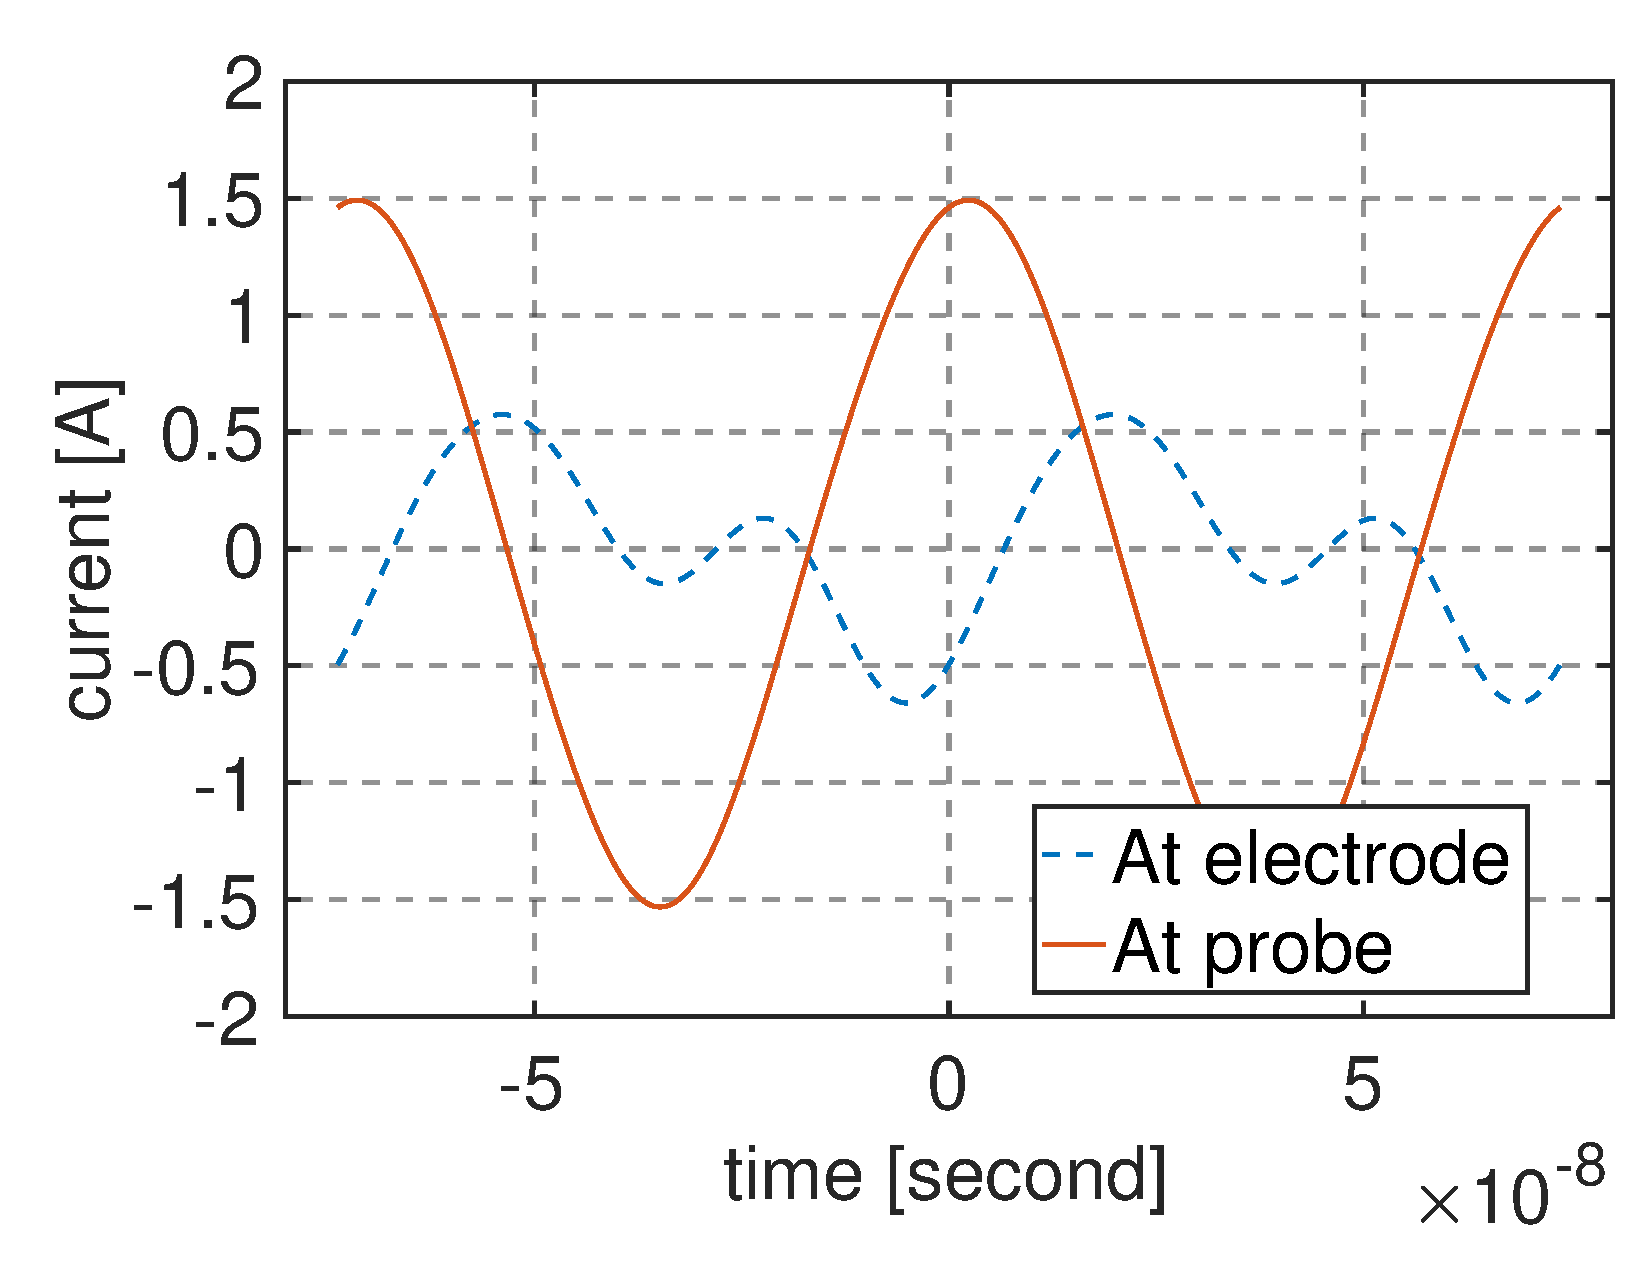
\includegraphics[width=1\textwidth]{electrode_vs_probe_current.pdf}
\end{minipage}
\begin{minipage}{0.495\textwidth}
    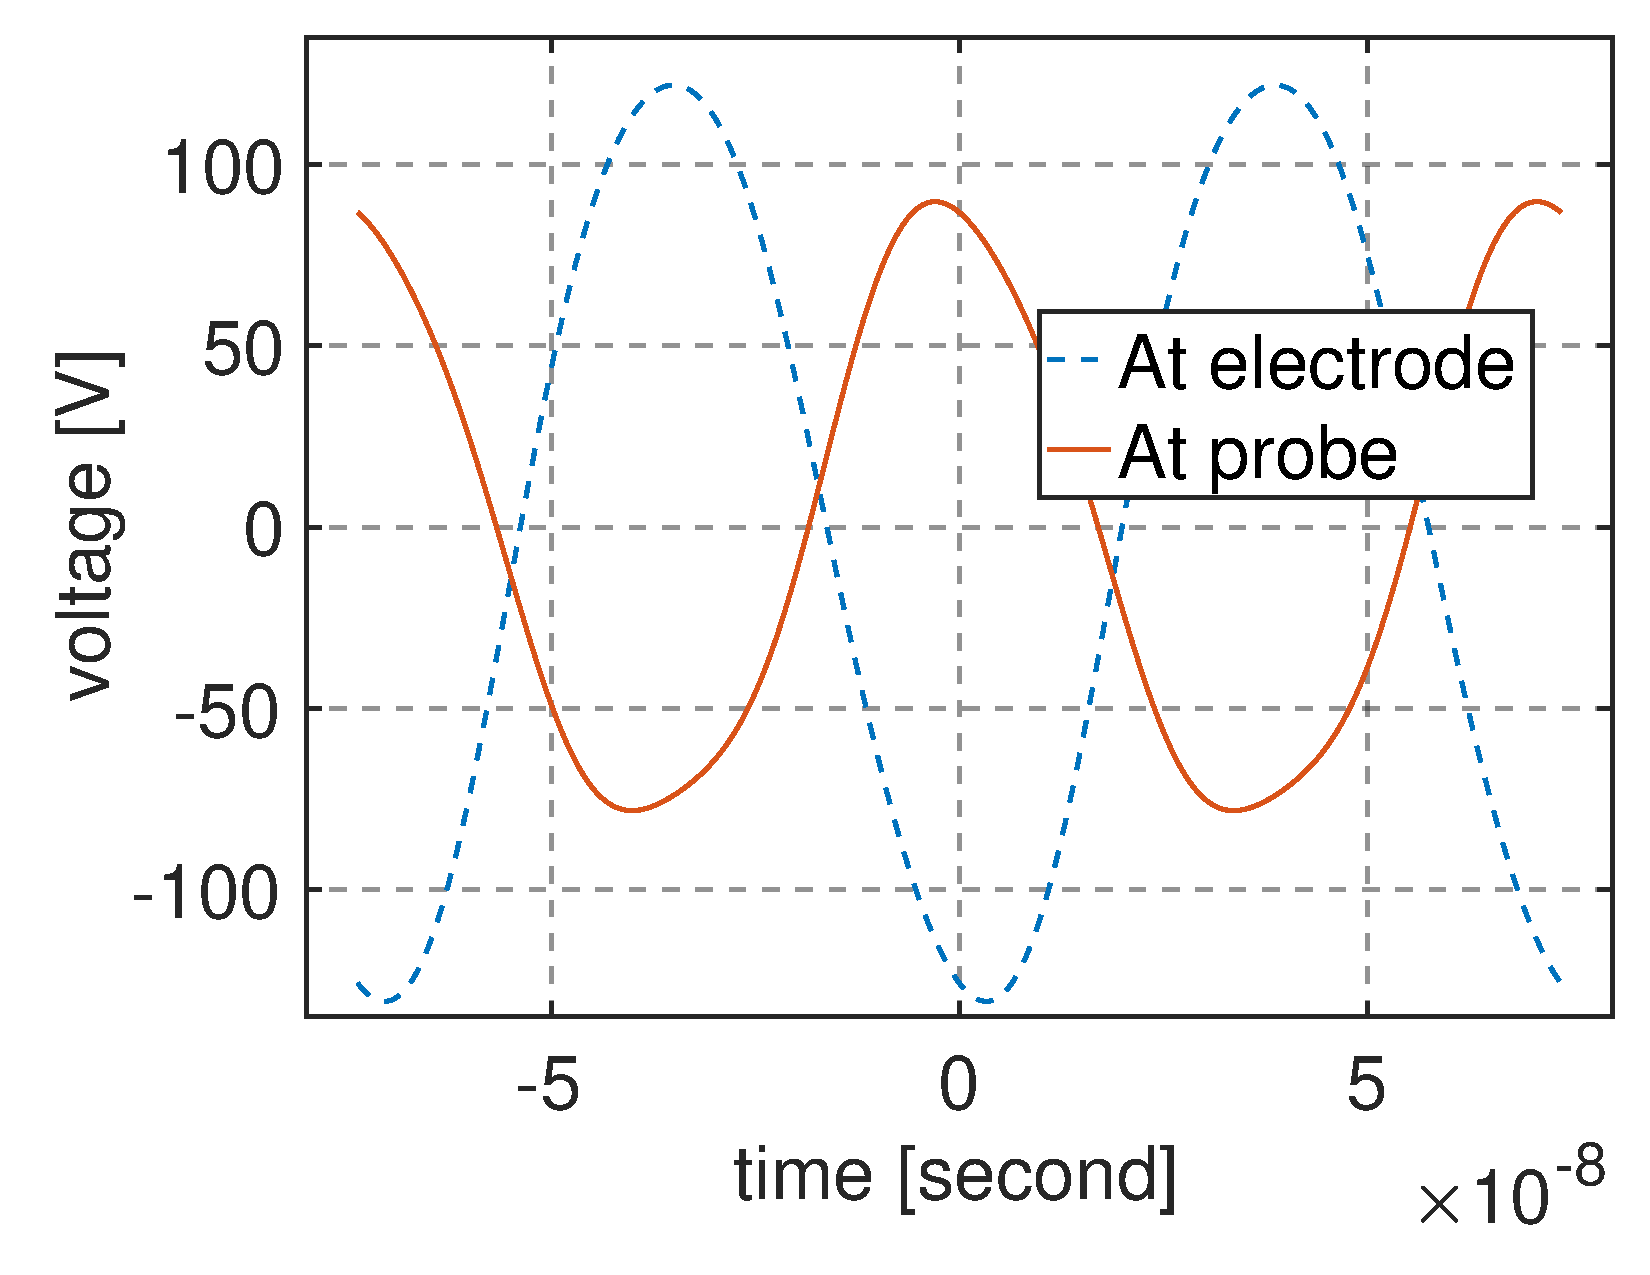
\includegraphics[width=1\textwidth]{electrode_vs_probe_voltage.pdf}
\end{minipage}
	\caption{Example (a) rf current (b) rf voltage traces measured at the probe and reconstructed at the electrode by correcting for parasitic impedances and transmission delay for a 0.5 Torr argon discharge. \textbf{IS THIS THE SAME FIGURE AS IN THE FIRST PAPER?  IF SO, THAT WILL NEED TO BE NOTED - OR BETTER YET, MAKE SOME CHANGES TO THE FIGURE SO THERE ARE NO COPYRIGHT INFRACTIONS.  - BUT STILL NOTE THAT IT IS THE SAME DATA...}}
	\label{Fig:Current_v_time}
\end{center}
\end{figure}


The current to the electrode consists of both conductive and displacement currents. Conductive current arises because the electrons are much lighter than the ions and thus can follow instantaneous changes in the potential profile of the plasma induced by the RF field. Since electrons have at least approximately a Maxwellian velocity distribution, the electron density at the electrode face, as well as the electron current $i_e$, follow the Boltzmann relation and decreases exponentially as the potential falls below the plasma potential in the sheath \cite{sobolewski1995electrical},
\begin{equation} 
    i_e=i_k\exp[e\phi\left(t\right)/k_B T_e],
    \label{eqn:electron conduction}
\end{equation}
where $T_e$ is the electron temperature, $k_B$ is Boltzmann's constant. $i_k$ is a function of bulk electron density and temperature \cite{sobolewski1995electrical} and $\phi\left(t\right)$ is the voltage across the sheath,
\begin{equation} 
    \phi\left(t\right) = -\phi_{dc} + \phi_1\cos(\omega t).
    \label{eqn:sheath voltage}
\end{equation}
Here $\phi_{dc}$ is the DC and $\phi_1\cos(\omega t)$, is the time varying voltage across the sheath, a portion of which is the applied RF voltage. While the electrons respond to the time dependent field, ions only respond to the time averaged potential and thus largely results in a dc current $i_{ion}$ which depends on the electrode area A, ion density $n_i\left(x\right)$ and velocity $u_i\left(x\right)$ at a distance x from the powered electrode \cite{sobolewski1995electrical},
\begin{equation} 
    i_{ion}=e\ n_i\left(x\right)u_i\left(x\right)\ A 
\end{equation} 
Thus, the total conduction current $i_c\left(t\right)$ is given by, 
\begin{equation}
i_c\left(t\right)=i_k\exp[e\phi\left(t\right)/k_BT_e]+i_{ion}
\label{eqn:conduction_current}
\end{equation}
In a similar fashion, displacement currents arise from the time variation of the sheath electric field.  Using the fact that the derivative of an even sinusoidal function is odd, one can separate the total current into its conduction and displacement components \cite{sobolewski1995electrical}. This can be easily seen from the definition of displacement current, 
\begin{eqnarray}
    i_d\left(t\right) &=\epsilon_0A\frac{d}{dt}[\phi \left(t\right)/ s\left(t\right)] \\
    &=\frac{\epsilon_0A} {s\left(t\right)}\frac{d\phi \left(t\right)}{dt}-\phi \left(t\right)\frac{\epsilon_0A}{s\left(t\right)^2}\frac{d}{dt}s\left(t\right)
\label{eqn:displacement_current}
\end{eqnarray}
where, $s\left(t\right)$ is the sheath thickness and A is the surface area of the electrode. If $\phi\left(t\right)$ is an expressed as an even sinusoidal function, $i_c$ is even whereas $i_d$ is odd, given that the sheath thickness is in phase with the applied voltage \cite{panagopoulos1999plasma}. One can use equation (\ref{eqn:sheath voltage}) to expand the electron conduction current from equation (\ref{eqn:electron conduction}) into a Fourier series,
\begin{eqnarray} 
    i_e &= i_k\exp[e\phi\left(t\right)/k_B T_e] \\
    &= i_k\exp [-e\phi_{dc}] \exp[ e\phi_1\cos(\omega t)/k_B T_e] \\
    &= i_{e,dc} + \sum^{\infty}_{n=1} i_{e,n} \cos(n\omega t)
\end{eqnarray}
With the coefficients, 

\begin{equation} 
    i_{e,dc} =  i_k \exp [-e\phi_{dc}] \frac{\omega}{\pi} \int^{\pi/\omega}_0 \exp[e\phi_1\cos(\omega t)/k_B T_e] dt
\end{equation}
And,
\begin{equation} 
    i_{e,n} = i_k \exp [-e\phi_{dc}]\frac{2\omega}{\pi} \int^{\pi/\omega}_0 \exp[e\phi_1\cos(\omega t)/k_B T_e] \cos(n\omega t) dt
\end{equation}
where, $n = 1,2,3..$. A similar Fourier expansion can be done for the displacement current to find the coefficient, $i_{d,n}$. As our probe only measures time varying current, we can calculate the currents at the fundamental and its harmonic frequencies namely $i_{e,n}$ and $i_{d,n}$, but not the time average electron current $i_{e,dc}$. However, since the time average of the conduction current $i_c$ is zero due to the blocking capacitor (Figure \ref{Fig:mGEC_Circuit}), we have from equation (\ref{eqn:conduction_current}),
\begin{equation}
i_{e,dc} = -i_{ion}
\end{equation}


\section{mGEC moderate pressure plasma Database}\label{Sect:Database}

A study of intermediate pressure plasma can consist of an indefinite number of experiments involving many variables such as feed gas, power, pressure, interelectrode gap, etc. We selected argon, nitrogen and oxygen and different mixtures of them as our feed gases. Argon is the most common noble gas used in plasma experiments and is a standard gas well suited for comparative study due to its prevalence in past research whereas nitrogen and oxygen are good representatives for electropositive and electronegative plasmas respectively. The nominal power for this study was kept within a hundred Watts while the operating pressure was kept between 0.5 and 2.5 Torr. The gap between the driven and the grounded electrode was kept between 20 and 28 mm since most industrial systems operate near that gap.

To understand the effects of these control parameters on the measured I-V data, a design of experiment (DOE) screening was developed using a commercial software package (JMP). The screening was done by varying the control parameters within a given range. Electrode gap variation was limited between 20 mm and 28 mm while power variation was done between 10 Watts and 70 Watts. Feed gases were also varied for this screening with pure argon, nitrogen and oxygen as well as mixtures of any two of those gases. Current and voltages were measured at random combinations of these four control parameters namely applied power, electrode gap, operating pressure, and ratio of feed gases. The experiments were repeated four times. The measured quantities were plotted against each control parameter and p-values were calculated to compare the fit between the control and measured parameters using JMP. Variation in electrode gap was found to have an insignificant correlation with all the measured quantities and thus was kept fixed at 24mm for subsequent experiments.  

\textbf{make a table of p-values for 3 control parameters vs. measurements}\\

\begin{table}[]
    \centering
%   \begin{tabular}{|c|c|c|c|c|c|c|}
\begin{tabular}{ |p{3.5cm}|p{1.5cm}|p{1.5cm}|p{1.5cm}|p{1.5cm}|p{1.5cm}|p{1.5cm}| }
        \hline
        Parameter & Ar flow (\%) & $N_2$ flow (\%) & $O_2$ flow (\%) & Pressure (Torr) & gap (mm) & Nominal power (Watts) \\
        \hline
        Powered electrode &&&&&&\\
        \hline
        $V_{DC}$ & 0.0024 & 0.0311 & 0.4070 & $<$0.0001 & 0.7025 & $<$0.0001\\
        $V_{rf,1}$ & 0.0012 & 0.0043 & 0.7295 & 0.0252 & 0.7869 & $<$0.0001\\
        $V_{rf,2}$ & 0.0001 & 0.0444 & 0.0971 & 0.0007 & 0.9940 & $<$0.0001\\
        $V_{rf,3}$ & 0.9278 & 0.8050 & 0.8758 & $<$0.0001 & 0.8299 & $<$0.0001\\
        $I_{rf,1}$ &  $<$0.0001 & 0.0083 & 0.0911 & 0.9634 & 0.8046 & $<$0.0001\\
        $I_{rf,2}$ & 0.0001 & 0.0450 & 0.0970 & 0.0007 & 0.9933 & $<$0.0001\\
        $I_{rf,3}$ & 0.8136 & 0.7093 & 0.8912 & $<$0.0001 & 0.8446 & $<$0.0001\\
        \hline
        Ground electrode &&&&&& \\
        \hline
        $I_{gnd,1}$ & 0.0009 & 0.0225 & 0.3313 & 0.0031 & 0.1812 & $<$0.0001\\
        $I_{gnd,2}$ & 0.3328 & 0.4769 & 0.7984 & $<$0.0001 & 0.3369 & $<$0.0001\\
        $I_{gnd,3}$ & 0.0585 & 0.1756 & 0.5999 & 0.0012 & 0.5578 & $<$0.0001\\
        \hline
    \end{tabular}
    \caption{p-values for control parameter effects on measured current and voltages.  It is noted that the observed p-value for gap is always large, indicating that the gap, over the range studied, is not important in the results. In light of this, the gap was not examined in much of the additional parameter sweeps.}
    \label{tab:DOE_Results}
\end{table}


 Once the screening was completed, comprehensive experiments were conducted across power, pressure and gas mixtures. Experiments were run for all combinations of pressure of 0.5, 1.5, 2.5 Torr, and nominal power of 10, 25, 40, 55, 70 Watts (read from the wattmeter) for pure argon, nitrogen, and oxygen as well different mixtures between them [ref-table]. Each experiment was run for a total of four times and 13 full RF cycles were processed for each run. Each cycle consisted of about 738 data points acquired by the oscilloscope giving a phase resolution of about one-half degree. A 13x4 matrix was built for all parameters of interest for each run. For each of the four iterations, average parameter values were calculated from the set of 13 acquired cycles. To study interpolation using machine learning, additional data were later collected at 1 Torr and 2 Torr for the same gap, gas mixtures and power ranges. Data at 1 and 2 Torr were collected only once and post-processed in a similar way.

\begin{table}[]
    \centering
%    \begin{tabular}{|c|c|c|}
\begin{tabular}{ |p{4cm}|p{4cm}|p{4cm}| }
        \hline
        Dataset 1 & Dataset 2 & Dataset 3 \\
        \hline
        Set 1: DOE data: RANDOM combinations of gap: 20 -28mm, power:10-70 W, pressure: 0.5 -2.5 Torr and gas mix: Ar:N2:O2 = 1:0:0, 1/3:2/3:0, 2/3:1/3:0… 9 possible ratios. Four total runs. & Set 2: Data at 24mm: ALL combinations of power: 10,25,40,55,70 W, pressure: 0.5, 1.5, 2.5 Torr and gas mix: Ar:N2:O2 = 1:0:0, 1/3:2/3:0, 2/3:1/3:0… all 9 ratios at gap 24mm. Four total runs. & Set 3: Extension of set 2 to include data at 1 and 2 Torr. Only 1 run. \\
        \hline
    \end{tabular}
    \caption{mGEC I-V database structure: Set of data collected over time starting with a DOE set (Dataset 1). A more comprehensive set of data was later collected based on the DOE study (Dataset 2). Finally, a third set of data was collected for interpolation studies (Dataset 3)}
    \label{tab:Datasets}
\end{table}


\textbf{make a table of all 40 variables. Classify according to first harmonic phase dependence, control parameters and measured/calculated parameters }\\


\begin{table}[]
    \centering
%    \begin{tabular}{|c|c|c|}
\begin{tabular}{|p{7cm}|p{7cm}|}
        \hline
        Variable name & Description\\ 
        \hline
    1. $Ar\ flow\%$, $N2\ flow\%$, $O2\ flow\%$ & Feed gas percentage \\
    2. $pressure\ Torr$ & Operating pressure\\
    3. $power\ W$ & Applied power (nominal)\\
    4. $gap(mm)$ & Gap between electrodes\\ 
       \hline
           \end{tabular}
    \caption{Control parameters}
    \label{tab:Control_parameters}
\end{table}

DC self bias as well as magnitude and phases of electrode voltage and currents were measured at the first three harmonics as a function of the control parameters. Power, impedance, conduction and displacement currents were calculated from the measured magnitude and phases. Measured phase for the fundamental component was found to have a high error bar due to tuning variability of the matching network [ref.paper1]. Three separate matrices were constructed from the available datasets (dataset 1, 2 and 3) for machine learning and statistical analysis with JMP. The first matrix consists of the first harmonic phase independent 26 parameters (e.g. voltage and current magnitudes and DC bias) from all three sets above. For the first two datasets mean of the four runs were used, size 291x26. The second matrix has all 34 parameters with only the experiment corresponding to max electrode power of the four runs for the first two sets, size 201x34. This matrix was prepared to represent the "best" of the four runs since power loss in the transmission line was minimum for this run. Finally, the third matrix consists of all 34 parameters from all three sets above including all four runs for dataset 1 and 2, size 894x34. This is the comprehensive matrix including all experimental data regardless of error bar magnitude.

\begin{table}[]
    \centering
%    \begin{tabular}{|c|c|c|}
\begin{tabular}{ |p{4cm}|p{4cm}|p{4cm}| }
        \hline
        Matrix 1 & Matrix 2 & Matrix 3 \\
        \hline
         with only phase independent 26 parameters as a function of the 4 control parameters (e.g. voltage and current magnitudes at all harmonics, both magnitude and phase dependent parameters at second and third harmonics and DC bias) from all three sets above. For the first two datasets mean of the four runs were used, size 291x26 &  all 34 (both phase independent and dependent) parameters as a function of the 4 control parameters with only the experiment corresponding to max electrode power of the four runs for the first two sets, size 201x34 & all 34 parameters (both phase independent and dependent) from all three sets above including all four runs for dataset 1 and 2, size 894x34.\\
        \hline
    \end{tabular}
    \caption{Matrices for ML and JMP studies }
    \label{tab:ML_matrices}
\end{table}


\section{ Supervised Regression Analysis}\label{Sect:RegressionAnalysis}

*** Questions for Shadhin: 

\begin{enumerate}
    \item Did you use full hyper-parameter optimization for methods 2 to 4, if so worth stating this. If not, worth using the full hyper-parameter optimization.
    \item In your legends perhaps just show 2 significant figures of the R value and also show how many records in each dataset.
    \item May I suggest that you make the axis text larger, in the title state the variable, use correct capitalization, always show units. 
    \item It is worth showing the quantile quantile plots.
    \item It is worth having a table showing the performance of all the models (like a league table) sorted so that the best-performing model is first and the worst is last.

\end{enumerate}


Four different regression models were compared to each other for the supervised regression studies namely, 1) a deep neural network with the Lavenberg- Marquerdt backpropagation (trainlm) [ref], 2) an ensemble tree method (Treebagger) [ref] 3) a Gaussian regression (fitrgp) [ref] and 4) a support vector regression model (fitrsvm) [ref]. These models were used to predict 9 different current and voltage parameters namely the peak-to-peak magnitude of the electrode voltages, powered electrode currents and ground electrode currents at the first three harmonics. The input variables were standardized and all the models were optimized during training. For example, the random forest model i.e. treebagger was optimized using quantile error and Bayesian optimization [ref]. The predictor importance object "oobPredictorDeltaEroor" in the "treebagger" function in MATLAB was used to infer minimum number of inputs required while predicting high-error bar parameters. On the other hand, the neural network model was optimized by cross validating 15\% of the data and testing 15\% of the data while the rest was used for training. Additionally, the depth of the neural network was determined by finding the number of hidden layers between 10 and 50 giving the least Mean Squared Error (MSE) for each parameter.

Both interpolation and extrapolation were studied using supervised regression models. For interpolation models were trained at 0.5, 1.5, and 2.5 Torr and tested at 1 and 2 Torr. For extrapolation, prediction accuracy was checked at both the high and low end of the pressure range, namely at 2.5 and 0.5 Torr. For the high-pressure extrapolation at 2.5 Torr, the models were trained with data at the lower pressures, and for low-pressure extrapolation at 0.5 Torr, the models were trained with data at the higher pressures. This was done to check how the models perform at a pressure where the physics may be different than where they were trained on. For predicting the first harmonic phase independent parameters, only the control parameters namely the gas ratio, electrode gap, pressure, and nominal power were used as inputs. Since these parameters have a low error bar, mean values of the measured parameters from matrix 1 were used for training and testing the machine learning models. On the other hand, all available data from the four repeated experiments (matrix 3) were used to train and predict the first harmonic phase and phase-dependent parameters as they may have a high error bar due to the large variation of phase between repeated runs as explained above. Training the models with data from all experiments enables them to learn from an increased number of observations as well as from additional input parameters. These additional inputs can be used given they can be predicted accurately beforehand. This allows one to use cumulative inputs with the help of predictor importance ranking by the random forest model until the desired prediction accuracy is achieved.

% These predictions can either be as a function of control parameters from matrix 1 or more cumulative parameters that were predicted with only control parameters as inputs.can be predicted accurately either with the control parameters as inputs or other parameters which are predicted  they can be predicted accurately from matrix 1 using only the control parameters as inputs. High error bar parameters, already predicted with high accuracy were also used as inputs for parameters where predictions lacked greater accuracy. Once the best performing model were identified, predictions were made at even higher (> 2.5) or lower (< 0.5) pressure where no experimental data is available. For this purpose, matrix 2 was used for training the model so that predictions are consisted with one set of data? 

\textbf{figures for only control params inputs}

\begin{figure}[ht!]
\begin{center}
\begin{minipage}{0.495\textwidth}
    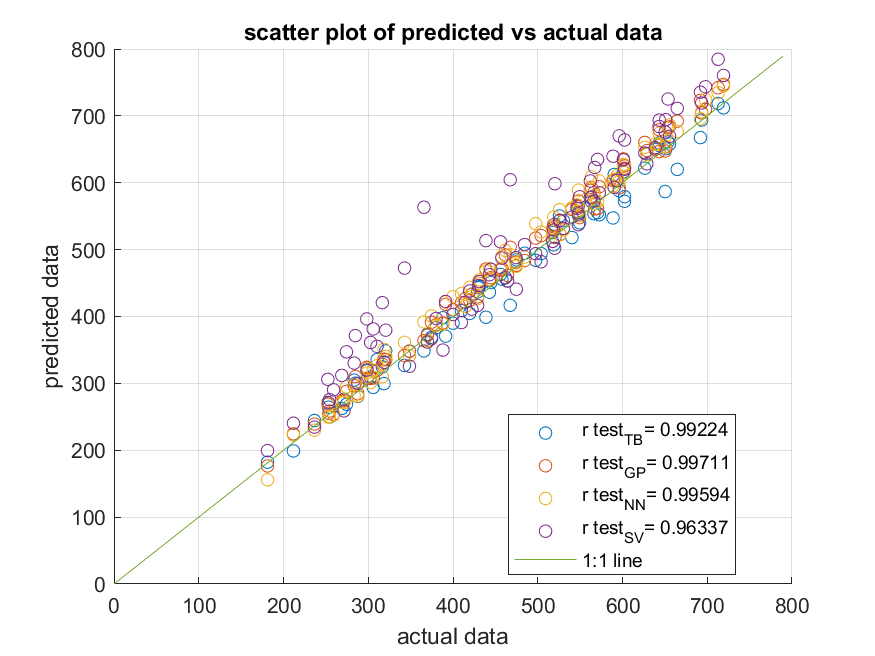
\includegraphics[width=1\textwidth]{volt1_12T.png}
\end{minipage}
\begin{minipage}{0.495\textwidth}
    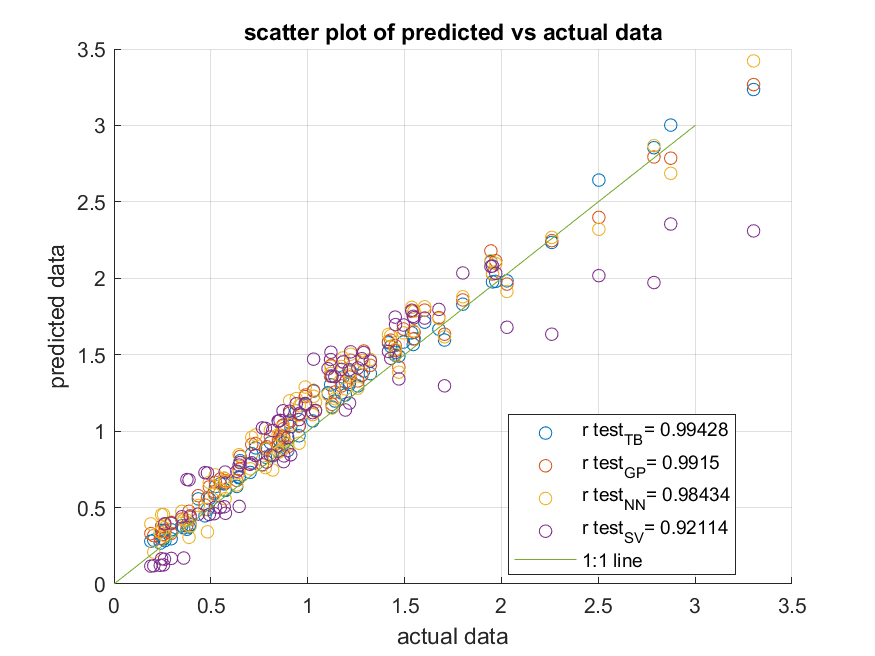
\includegraphics[width=1\textwidth]{current1_12T.png}
\end{minipage}
\begin{minipage}{0.495\textwidth}
    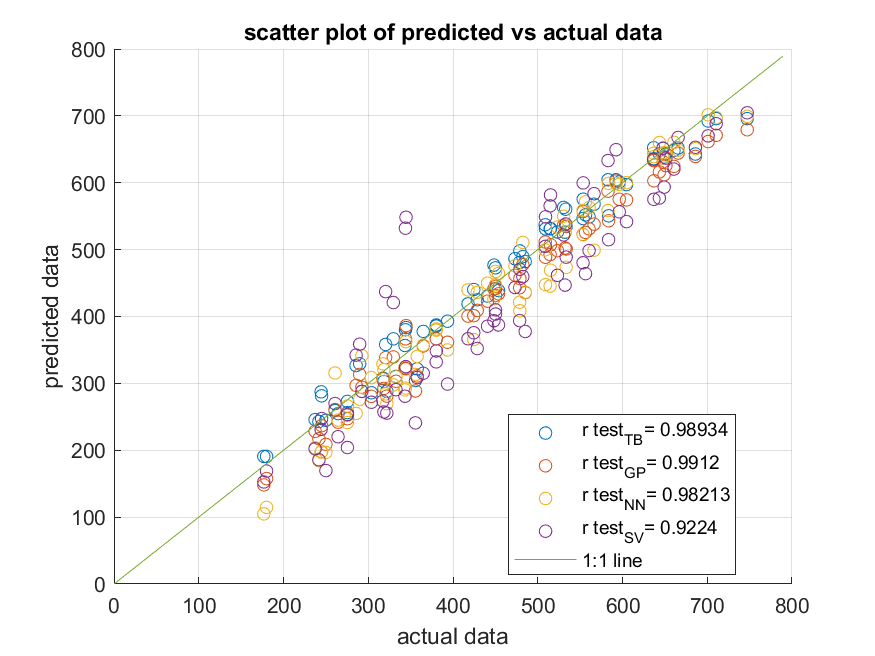
\includegraphics[width=1\textwidth]{volt1_2.5T.png}
\end{minipage}
\begin{minipage}{0.495\textwidth}
    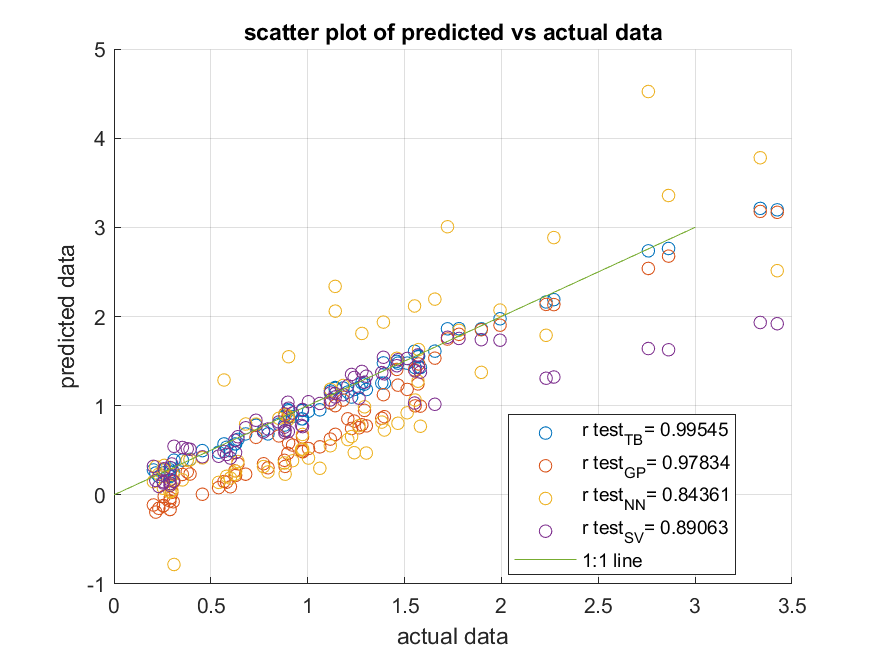
\includegraphics[width=1\textwidth]{current1_2.5T.png}
\end{minipage}
\begin{minipage}{0.495\textwidth}
    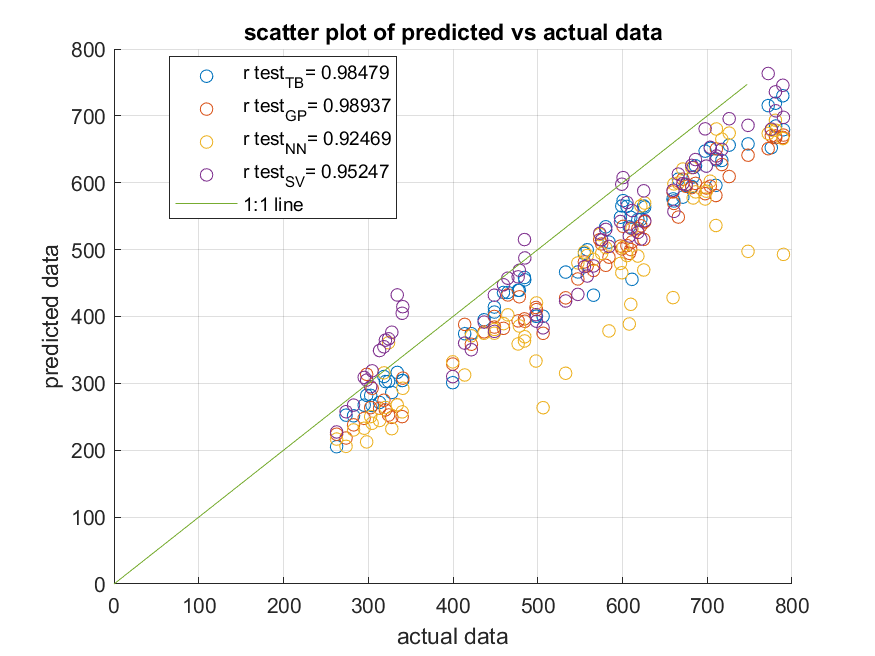
\includegraphics[width=1\textwidth]{volt1500mT.png}
\end{minipage}
\begin{minipage}{0.495\textwidth}
    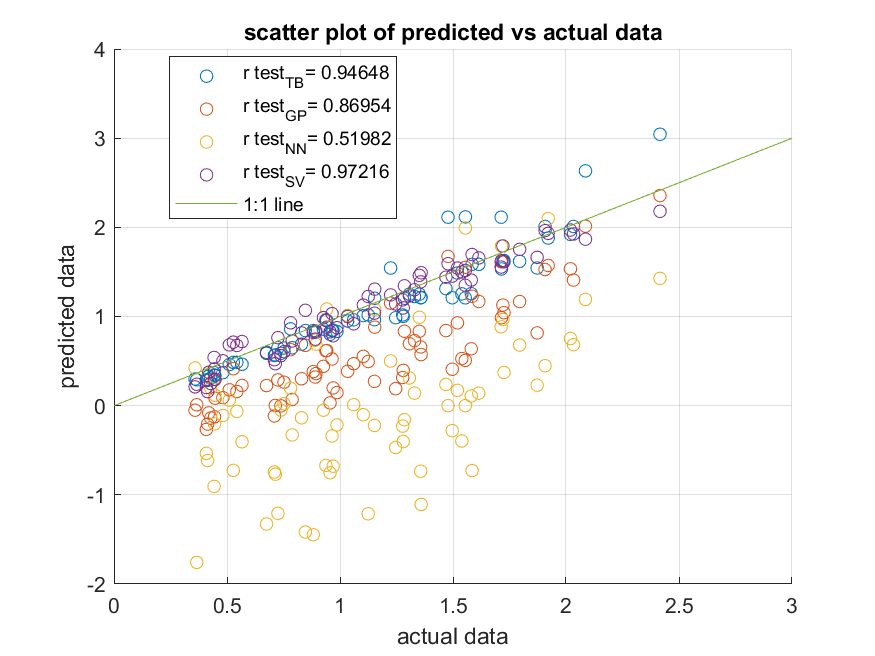
\includegraphics[width=1\textwidth]{current1500mT.png}
\end{minipage}

\caption{Interpolation and extrapolation prediction accuracy for fundamental voltage and current to the driven electrode at 1-2 Torr (top left and right), at 2.5 Torr (middle left and right) and 0.5 Torr (bottom left and right) } 

\label{Fig:gap_SV,pressure_TB,species_TB}
\end{center}
\end{figure}

First harmonic phase independent parameters were first examined by means of prediction with both interpolation and extrapolation. Matrix 1 was used to predict and check fit for the parameters at 1 and 2 Torr. 201 observations were used for training (201 x 6 matrix as input of the dataset) and predictions were checked against 90 observations at 1 and 2 Torr. Similarly, for extrapolation at 2.5 Torr and 0.5 Torr, 216 observations were used for training and predictions were checked against 75 observations. Voltage and currents to both powered and grounded electrodes at first and second harmonics were found to have a correlation coefficient of 0.95 or higher between the measured and predicted data by at least one model. The only exception was the second harmonic current to the ground electrode at 0.5 Torr with a correlation coefficient of 0.88. Predictions for the third harmonic values despite having a low error bar, for most cases were less accurate (r<0.95).

%Extrapolation (with available data) for low error bar parameters at 2.5 Torr and 0.5 Torr: Use matrix 1 to predict and check fit for measurements with low error bar (first harmonic phase independent parameters) at 2.5 Torr from models trained at lower pressures (0.5, 1, 1.5 and 2 Torr). Same was done to predict and check fit at 0.5 Torr from models trained at higher pressures (1, 1.5, 2 and 2.5 Torr). Only the control parameters: gas ratio, electrode gap, pressure, nominal power  were used as inputs (216 x 6 matrix as input of the dataset) and predictions were checked against 75 observations for both cases. The number of parameters with a correlation coefficient of 0.95 or higher between the actual and predicted data by at least one model were () for the first case and () for the second case. 

\textbf{figure of predict conduction current/phase with only CP vs with additional params}

\begin{figure}[ht!]
\begin{center}

\begin{minipage}{0.495\textwidth}
    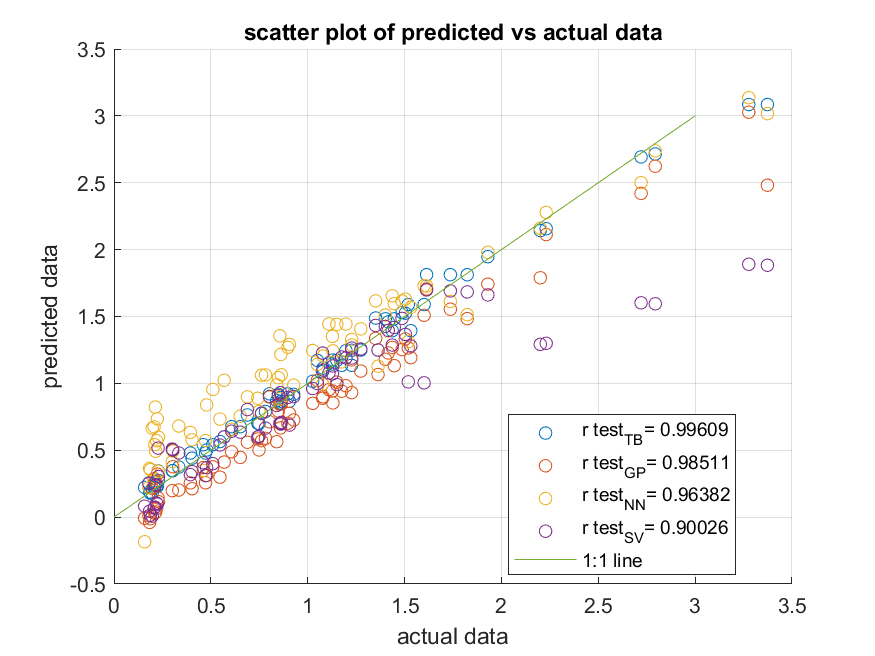
\includegraphics[width=1\textwidth]{dispWcontrol.png}
\end{minipage}
\begin{minipage}{0.495\textwidth}
    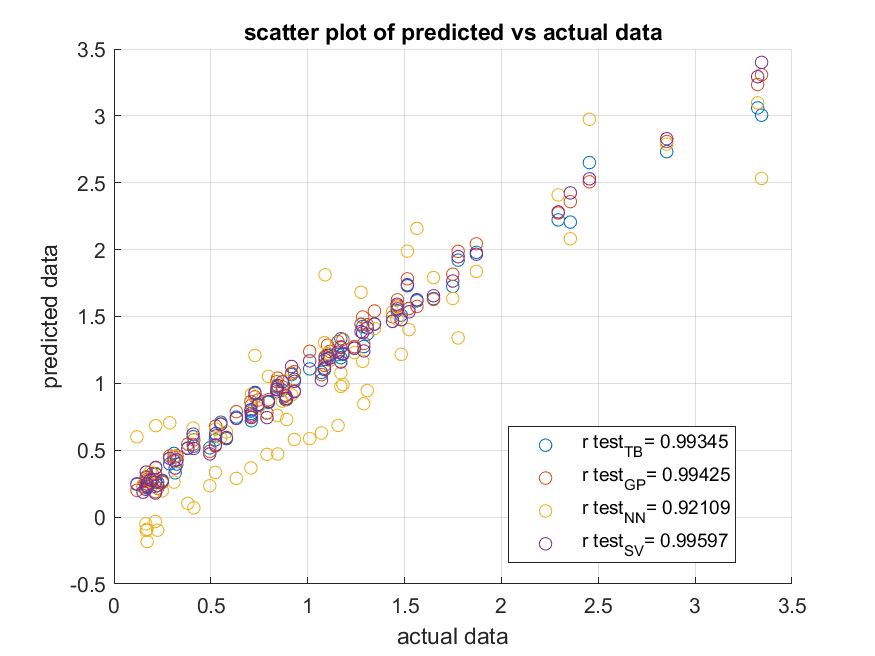
\includegraphics[width=1\textwidth]{disp.png}
\end{minipage}
\begin{minipage}{0.495\textwidth}
    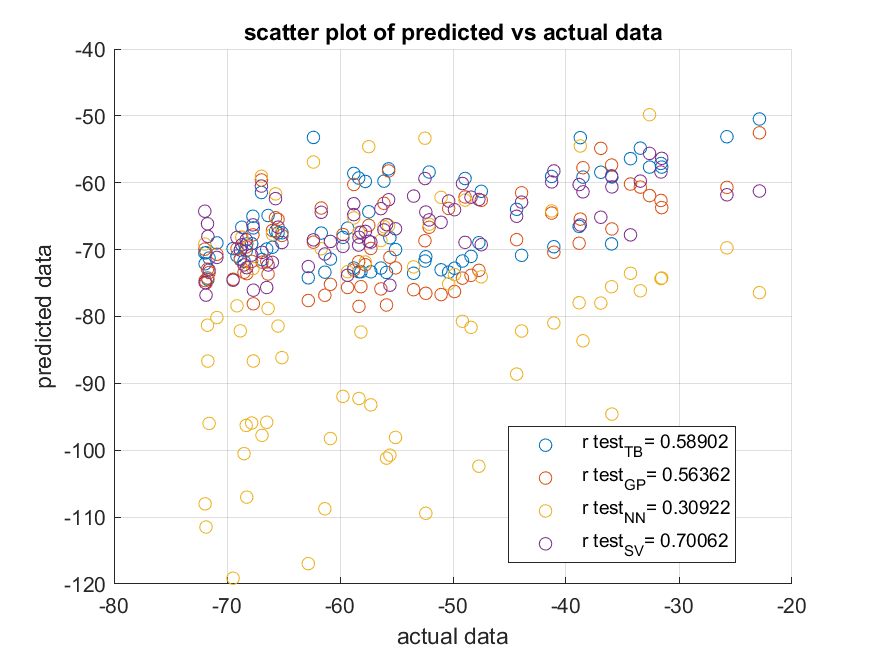
\includegraphics[width=1\textwidth]{phaseWcontrol.png}
\end{minipage}
\begin{minipage}{0.495\textwidth}
    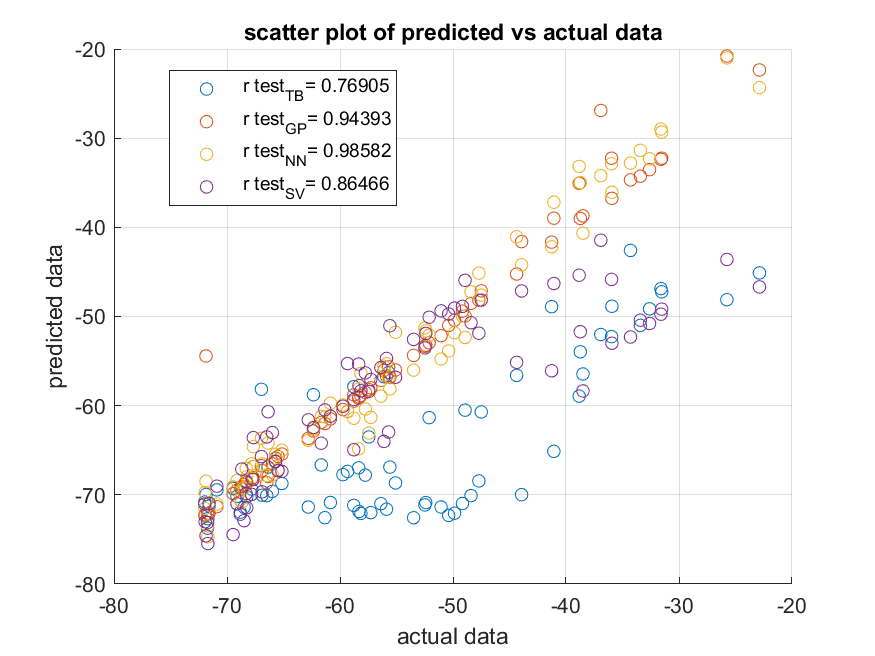
\includegraphics[width=1\textwidth]{phase.png}
\end{minipage}


\caption{Extrapolation of displacement current at 2.5 Torr with only control parameters (top left) vs. with total current as additional input (top right).Extrapolation of electrode phase at 2.5 Torr with only control parameters (bottom left) vs. with total and displacement current as additional inputs (bottom right)} 

\label{Fig:gap_SV,pressure_TB,species_TB}
\end{center}
\end{figure}

Interpolation and extrapolation were studied for first harmonic phase-dependent parameters as well, specifically the phase difference, conduction and displacement current at the powered electrode. For interpolating these parameters at 1 and 2 Torr, Matrix 3 was used to predict and check fit against 90 observations at 1 and 2 Torr, with models trained from 804 observations at 0.5, 1.5 and 2.5 Torr. And for extrapolation at 2.5 and 0.5 Torrs, 594 observations were used for training and 300 observations for testing. When using only the control parameters as inputs, only the displacement current predictions were accurate with a correlation coefficient >0.95. Although displacement current depends on phase, having a low error bar could explain its prediction accuracy with only control parameters as inputs. Due to the slope of cosine being small at measured phases of the cycle [footnote], the variation in displacement current is less sensitive to change in phase resulting in a lower error bar. Nonetheless, prediction accuracy was seen to increase even more with fundamental current as an additional input. First harmonic current to the powered electrode was chosen as the additional input since it was ranked as the most important predictor by the random forest for both interpolation and extrapolation cases. Once the total and displacement currents were predicted accurately, high error bar parameters like conduction current and phase were predicted next. Prediction accuracy for high error bar parameters was less accurate with only the control parameters as inputs. But with total and displacement currents as additional inputs, machine learning models were able to predict conduction current and phase with great accuracy (r>0.95 for most cases). This is not surprising given the fact that conduction current or phase can be easily calculated in a single step [footnote] with the knowledge of total and conduction currents beforehand.
%The only exception to this was the first harmonic electrode phase at 1-2 Torr with a correlation coefficient of r=0.86.

%Nonetheless, the use of cumulative input parameters with the help of predictor importance ranking, eventually resulted in greater prediction accuracy for conduction currents as well as phases.

\textbf{figures for conduction/phase with additional params}

\begin{figure}[ht!]
\begin{center}
\begin{minipage}{0.495\textwidth}
    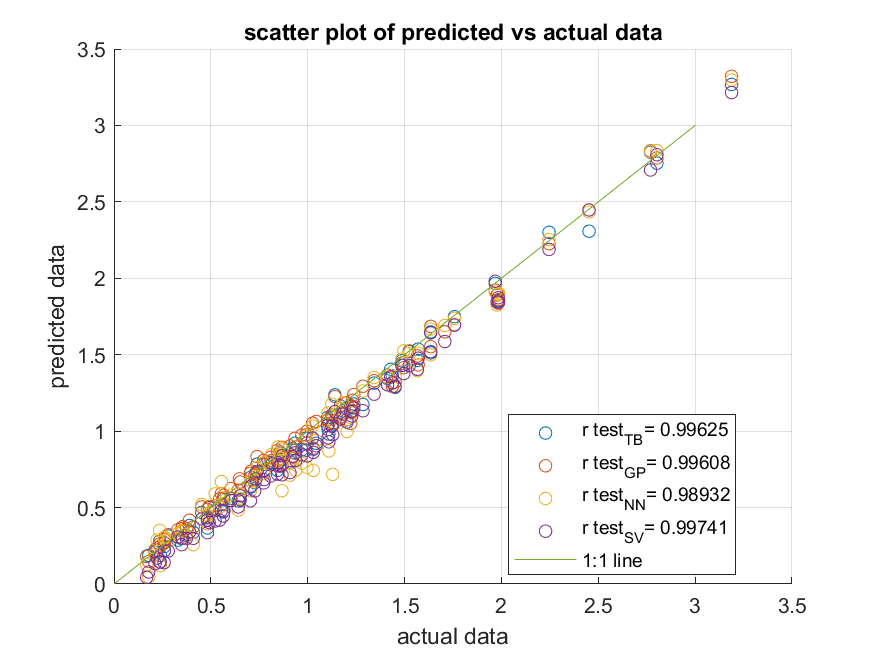
\includegraphics[width=1\textwidth]{disp_12T.png}
\end{minipage}
\begin{minipage}{0.495\textwidth}
    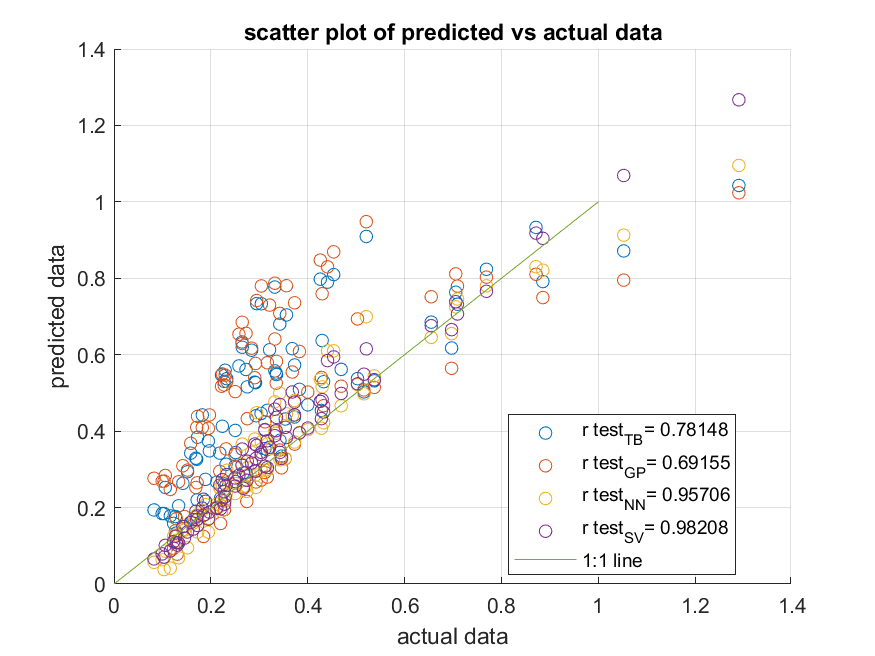
\includegraphics[width=1\textwidth]{cond_12T.png}
\end{minipage}
\begin{minipage}{0.495\textwidth}
    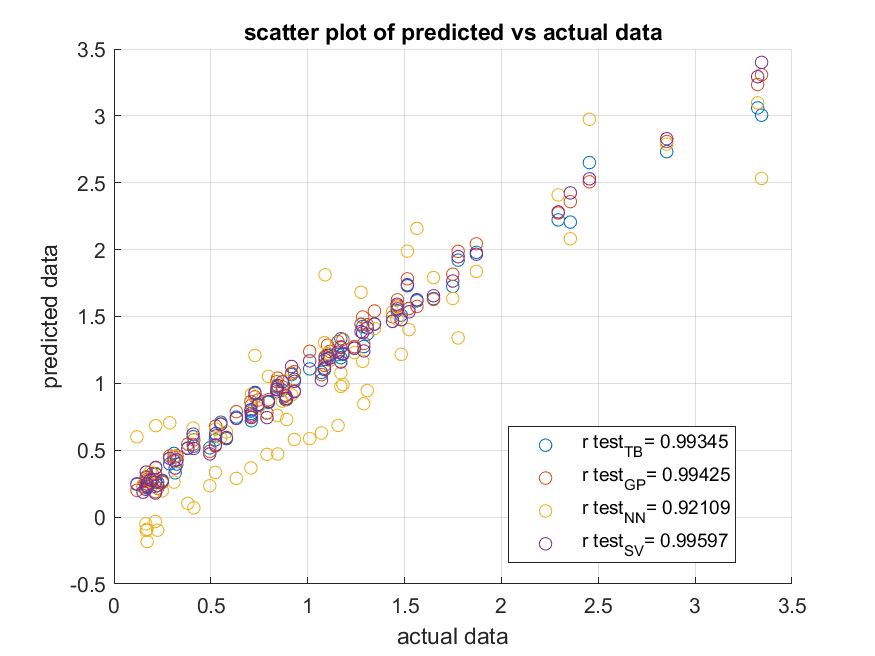
\includegraphics[width=1\textwidth]{disp_2.5T.png}
\end{minipage}
\begin{minipage}{0.495\textwidth}
    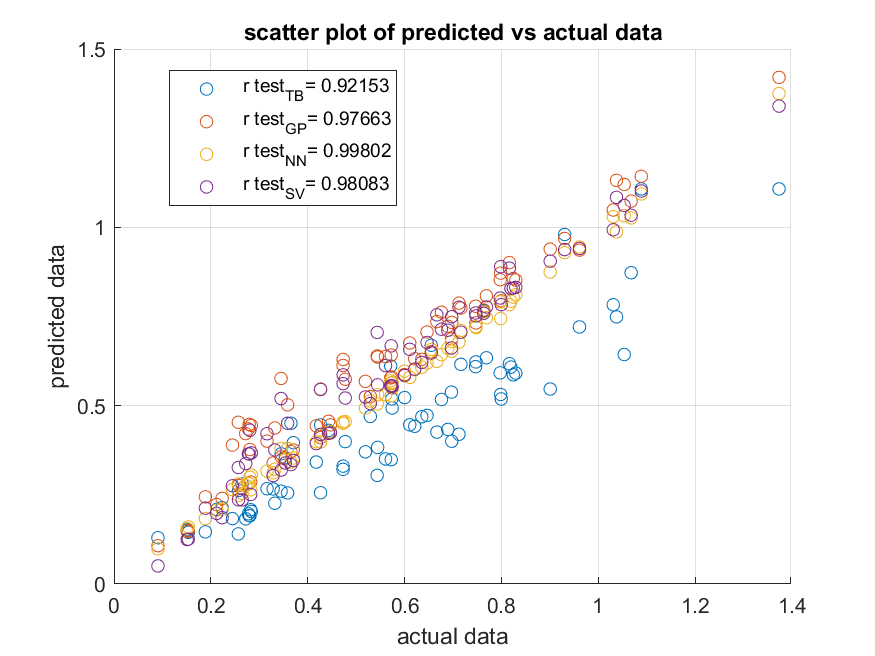
\includegraphics[width=1\textwidth]{cond_2.5T.png}
\end{minipage}
\begin{minipage}{0.495\textwidth}
    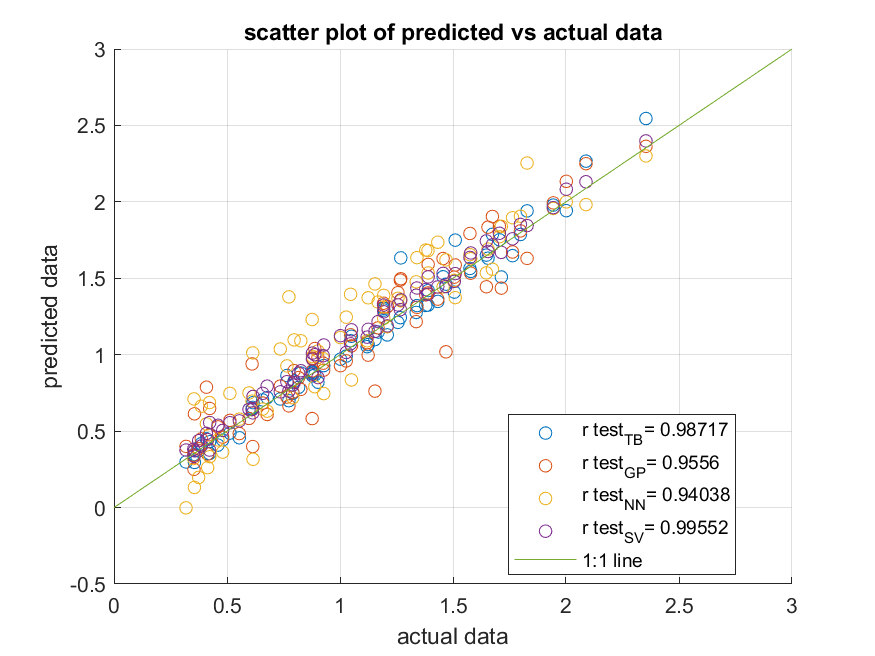
\includegraphics[width=1\textwidth]{disp_500mT.png}
\end{minipage}
\begin{minipage}{0.495\textwidth}
    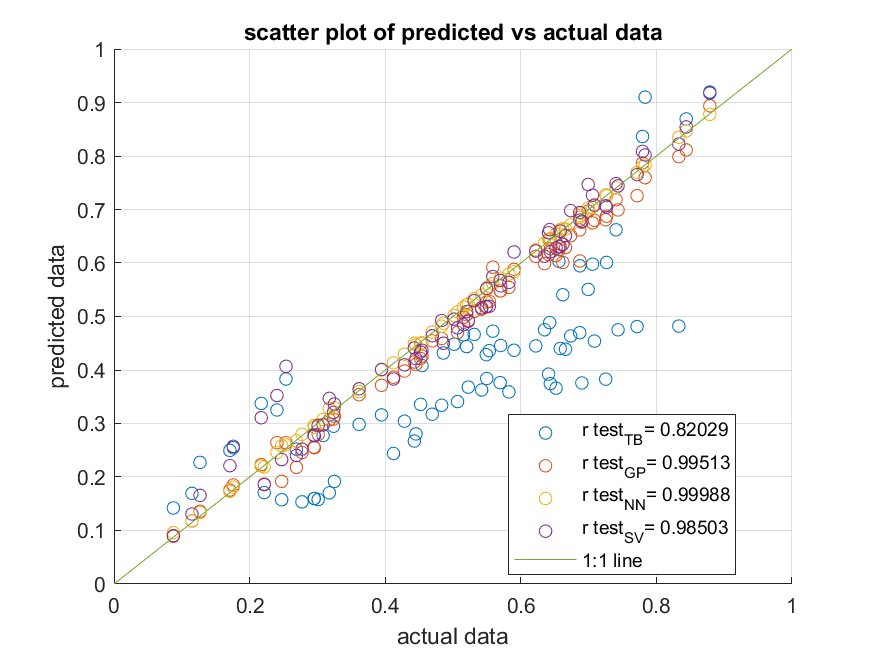
\includegraphics[width=1\textwidth]{cond500mT.png}
\end{minipage}

\caption{Interpolation and extrapolation prediction accuracy for displacement and conduction currents to the driven electrode at 1-2 Torr (top left and right), at 2.5 Torr (middle left and right) and 0.5 Torr (bottom left and right) } 

\label{Fig:gap_SV,pressure_TB,species_TB}
\end{center}
\end{figure}


% Interpolation at 1 and 2 Torr for high error bar parameters: Use table 3 to Predict and check fit for measurements with high error bars (first harmonic phase dependent parameters) at 1 and 2 Torr (90 observation for testing) using all parameters having a good predicted fit (correlation coefficient >0.95) at 1 and 2 Torr as inputs along with the control parameters (804 observations for training).  Both conduction and displacement current and phase data were predicted with a correlation coefficient of () by at least one model. The best-performing models were (). Minimize the number of inputs other than the control parameters based on the ranking of input parameter importance given by the random forest model training.

% Extrapolation (with available data) for high error bar parameters at 2.5 Torr and at 0.5 Torr: Use table 3 to Predict and check fit for measurements with high error bars (first harmonic phase dependent parameters) at 2.5 Torr (300 observation for testing) using all parameters having a good predicted fit (correlation coefficient >0.95) at 2.5 Torr as inputs along with the control parameters (594 observations for training). All predicted low error bar parameters at 2.5 and 0.5 Torr with a good prediction accuracy were used as inputs at first but only the ones needed to give a prediction accuracy 0.98 or higher were kept based on the predictor importance ranking from the random forest model. Displacement current was predicted with a correlation coefficient of .. by the model.. Although displacement current was predicted accurately with only the control parameters and low error bar parameters as inputs, conduction current and phase data predictions were not as good. Nonetheless, conduction current prediction accuracy was increased substantially when displacement current was used as one of the inputs. Models were trained at lower pressures (0.5, 1, 1.5 and 2 Torrs). Similarly, predict and check fit at 0.5 Torr from models trained at higher pressures (1, 1.5, 2 and 2.5 Torr). Both conduction and displacement current and phase data were predicted with a correlation coefficient of () by at least one model. The best performing models were (). 


Once extrapolation accuracy was checked at the high and low end of the pressure range namely 2.5 and 0.5 Torrs, one can further extrapolate where experimental data is unavailable. Matrix 2 was used to predict fundamental voltage and currents (total, conduction and displacement currents) at pressures greater than 2.5 Torr and smaller than 0.5 Torr. Predictions were made at 3.5 Torr with the model and inputs for that model giving the best fit at 2.5 Torr. The best model was trained for each respective parameter with all available data for that parameter at 0.5, 1 , 1.5, 2 and 2.5 Torr. Similarly, predict them at 0.1 Torr using the best-fitting model at 0.5 Torr. Predictions at 3.5 and 0.1 Torr were then compared with experimental I-V curves at 0.5, 1, 2, and 2.5 Torrs. ML predictions were found to be congruent with the experimental I-V trends at increasing/decreasing pressure.

\textbf{plots for experimental and ML comparison}

\begin{figure}[ht!]
\begin{center}
\begin{minipage}{0.495\textwidth}
    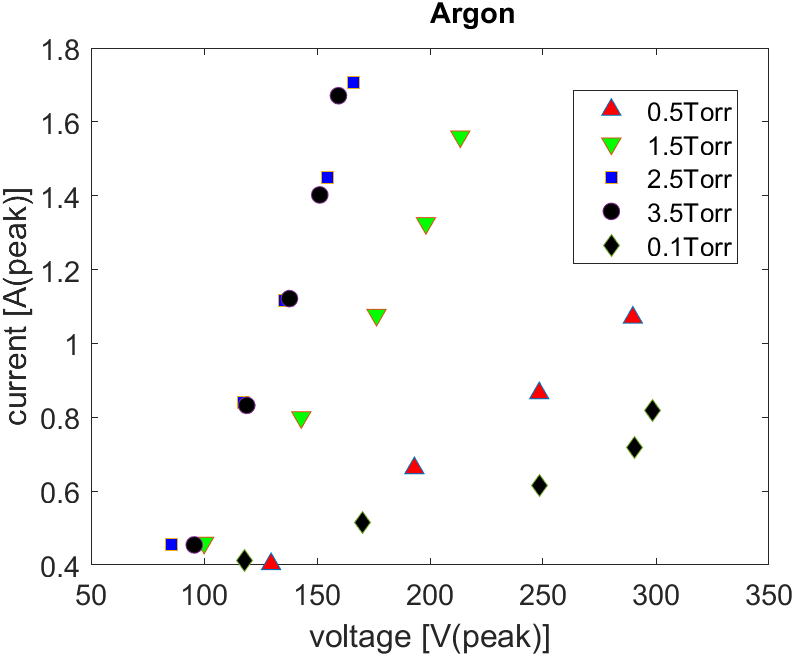
\includegraphics[width=0.8\textwidth]{Ar_current_volts.png}
\end{minipage}
\begin{minipage}{0.495\textwidth}
    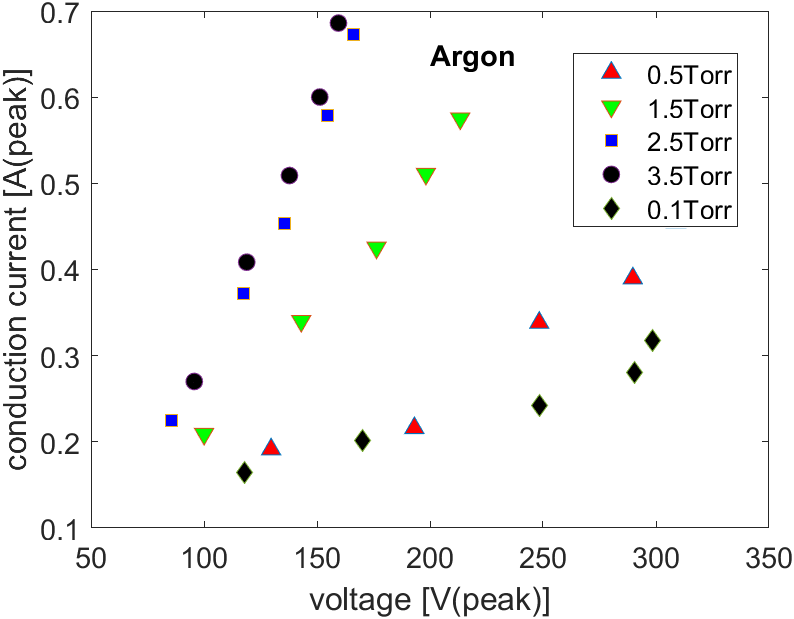
\includegraphics[width=0.8\textwidth]{Ar_conduction_volts.png}
\end{minipage}
\begin{minipage}{0.495\textwidth}
    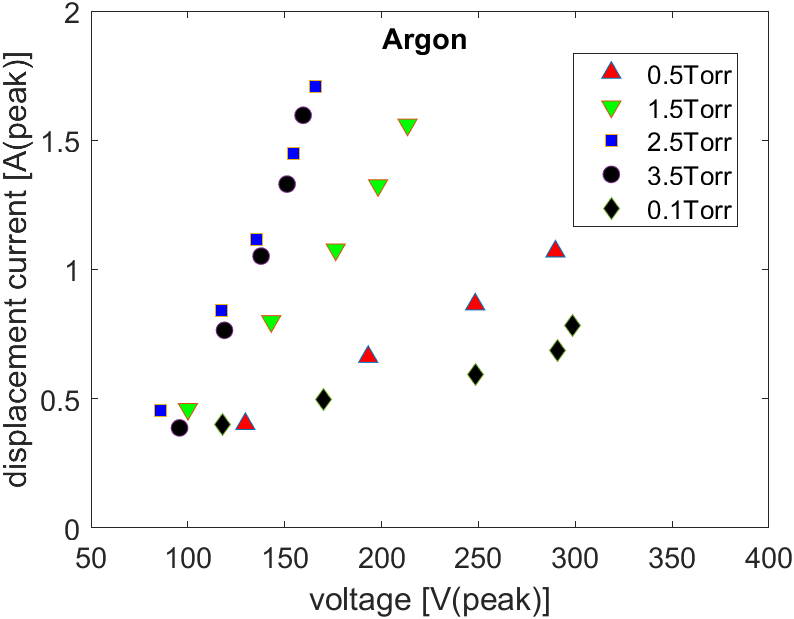
\includegraphics[width=0.8\textwidth]{Ar_disp_volts.png}
\end{minipage}
\begin{minipage}{0.495\textwidth}
    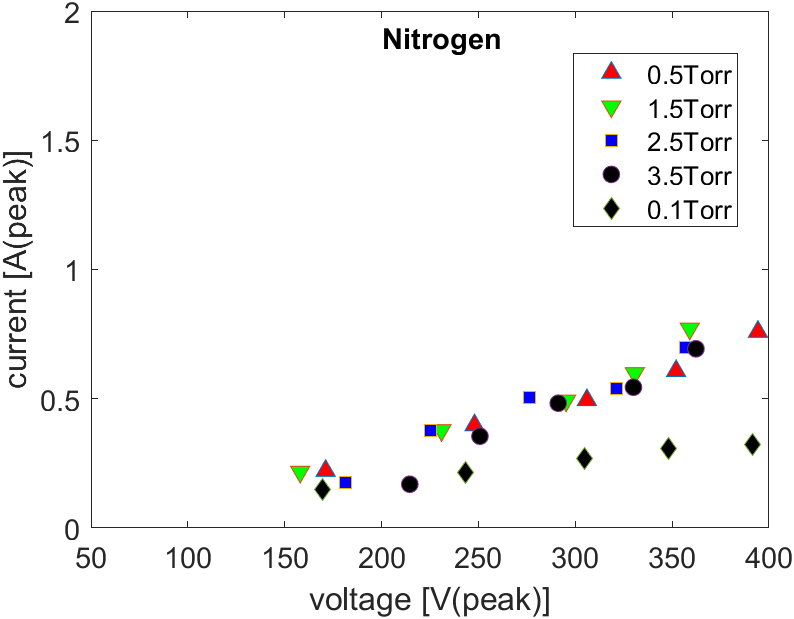
\includegraphics[width=0.8\textwidth]{N2current_volts.png}
\end{minipage}
\begin{minipage}{0.495\textwidth}
    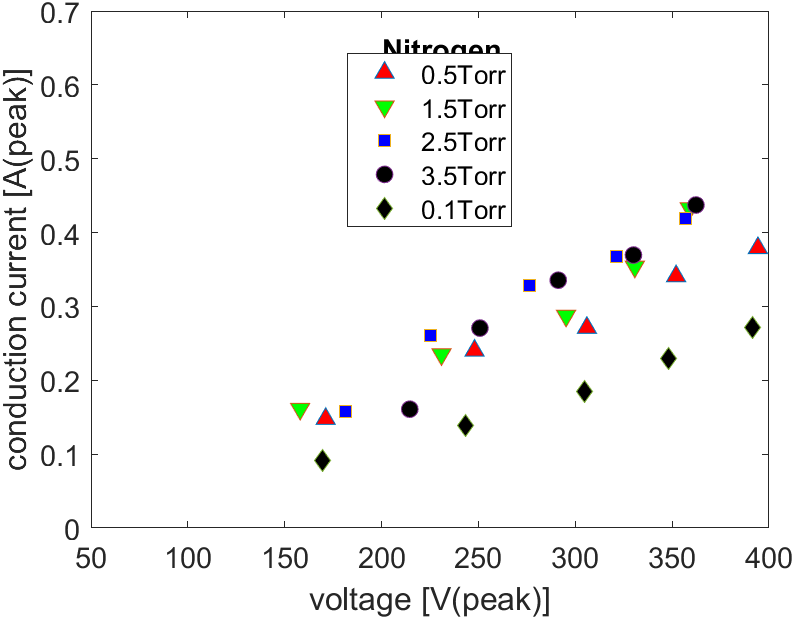
\includegraphics[width=0.8\textwidth]{N2conduction_volts.png}
\end{minipage}
\begin{minipage}{0.495\textwidth}
    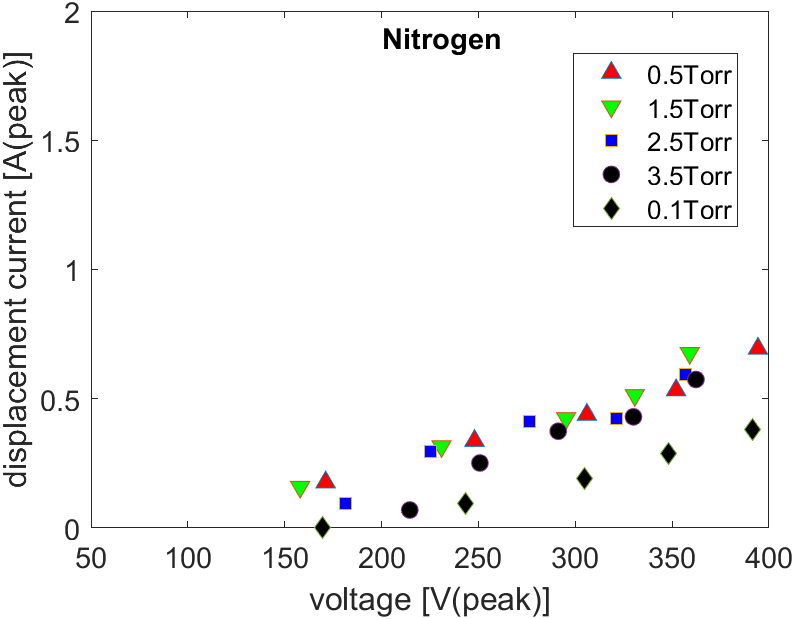
\includegraphics[width=0.8\textwidth]{N2disp_volts.png}
\end{minipage}
\begin{minipage}{0.495\textwidth}
    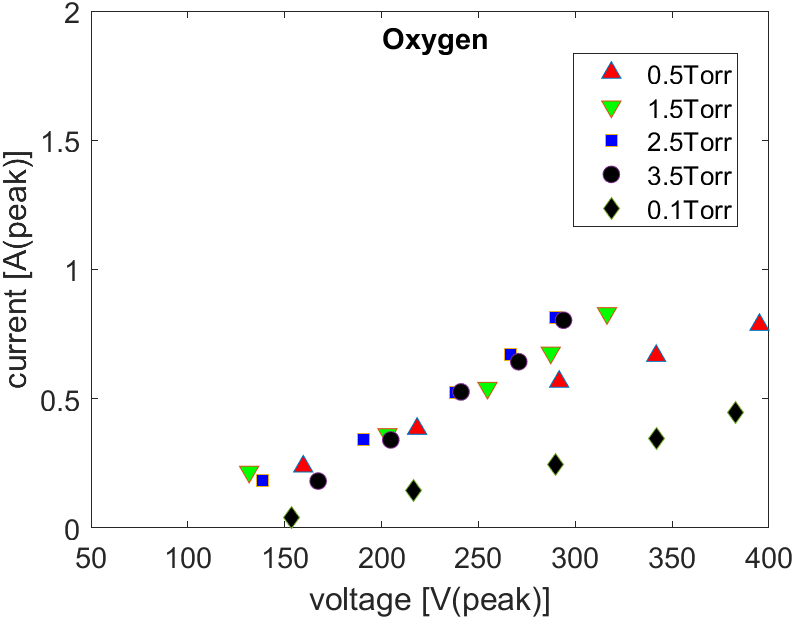
\includegraphics[width=0.8\textwidth]{O2current_volts.png}
\end{minipage}
\begin{minipage}{0.495\textwidth}
    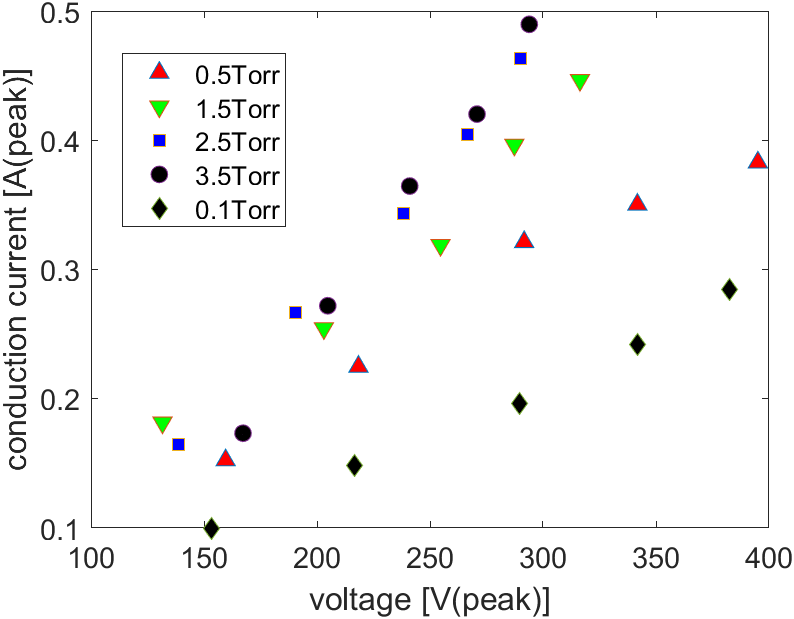
\includegraphics[width=0.8\textwidth]{O2conduction_volts.png}
\end{minipage}
\begin{minipage}{0.495\textwidth}
    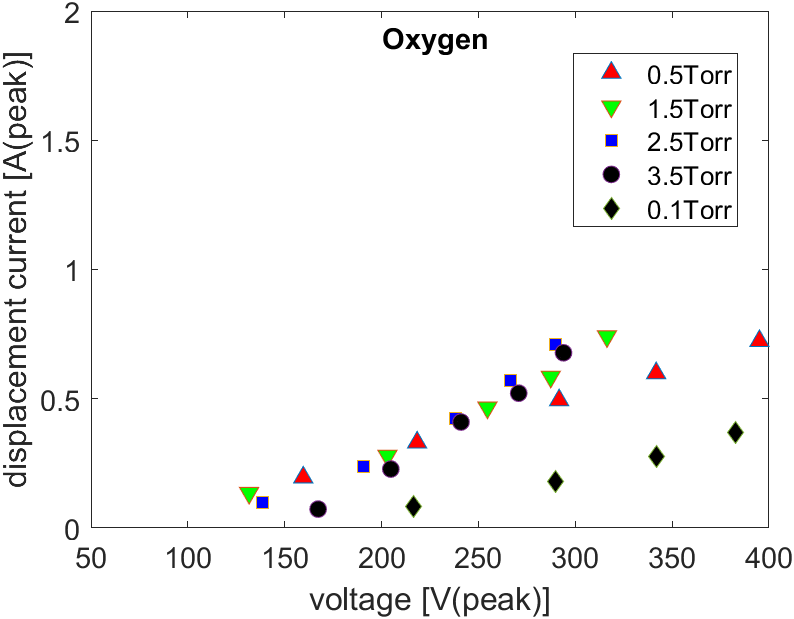
\includegraphics[width=0.8\textwidth]{O2disp_volts.png}
\end{minipage}

\caption{} 

\label{Fig:gap_SV,pressure_TB,species_TB}
\end{center}
\end{figure}



%Extrapolation (with NO available data) for low error bar parameters at higher (>2.5 Torr) and lower(<0.5 Torr) pressures: Choose the parameters with good fit (correlation coefficient >0.95) at 2.5 Torr and for each of those parameters use the model giving the best fit at 2.5 Torr. Train the model for each respective parameter with all available data for that parameter at 0.5, 1 , 1.5, 2 and 2.5 Torr and predict them at higher pressures (> 2.5 Torr) (75 x 10 matrix as output of the dataset) using matrix 2 (why?) with only the control parameters as inputs (291 x 6 matrix as input of the dataset). Similarly, predict them at lower pressures (<0.5 Torr) using the best fitting model at 0.5 Torr.

%Extrapolation (with NO available data) for high error bar parameters at higher (>2.5 Torr) and lower (<0.5 Torr) pressures: Use table 2 to predict high error bar parameters at higher pressures (>2.5 Torr), with the model and minimum number of inputs for that model giving the best fit at 2.5 Torr. Similarly, predict them at lower pressures (<0.5 Torr) using the best fitting model at 0.5 Torr. 


\textbf{report r-coefficient and MSerror for all predicted parameters for all 4 models?} 

%\subsection{interpolation accuracy at 1 and 2 Torr}
%\subsection{extrapolation accuracy testing for magnitude and phase at 2.5Torr }
%\subsection{prediction using control parameters}
%\subsection{increasing prediction accuracy with added features}
%\subsection{predicting phase and phase dependent variables}
%\subsection{extrapolation at pressures beyond 2.5}

\section{Classification of control parameters}\label{Sect:Classification}


\begin{figure}[ht!]
\begin{center}
\begin{minipage}{0.5\textwidth}
    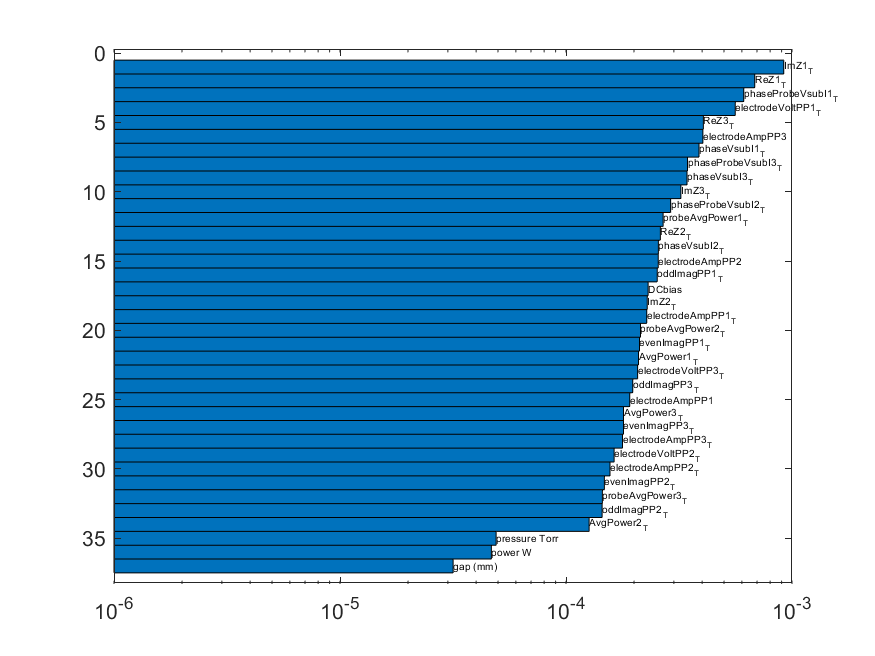
\includegraphics[width=1\textwidth]{input-importance-curvature-testSpecies.png}
\end{minipage}
\begin{minipage}{0.5\textwidth}
    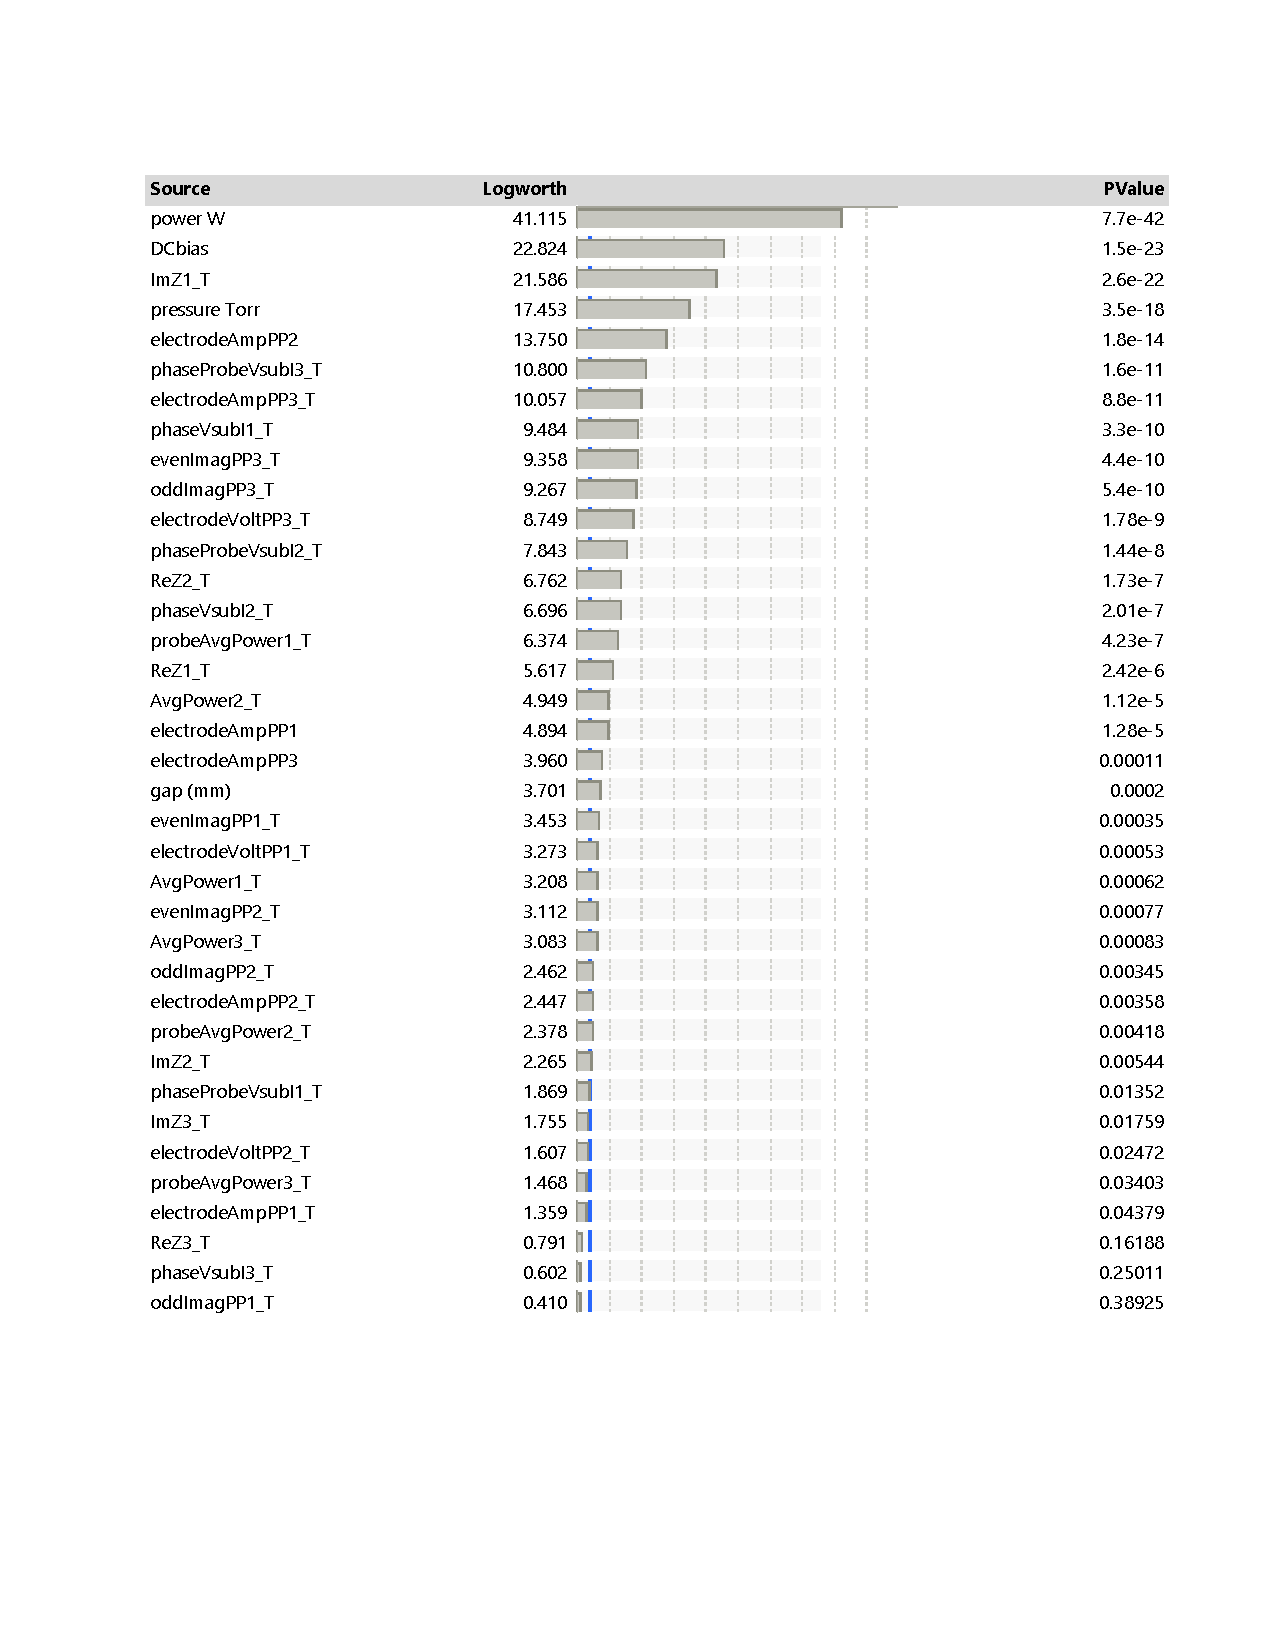
\includegraphics[width=1\textwidth]{jmpSpecies.pdf}
\end{minipage}

\caption{Predictor importance ranking for feed gas by random forest (top), p-value ranking of input parameters for least square fitting feed gas  (bottom) } 

\label{Fig:gap_SV,pressure_TB,species_TB}
\end{center}
\end{figure}

\begin{figure}[ht!]
\begin{center}
\begin{minipage}{0.5\textwidth}
    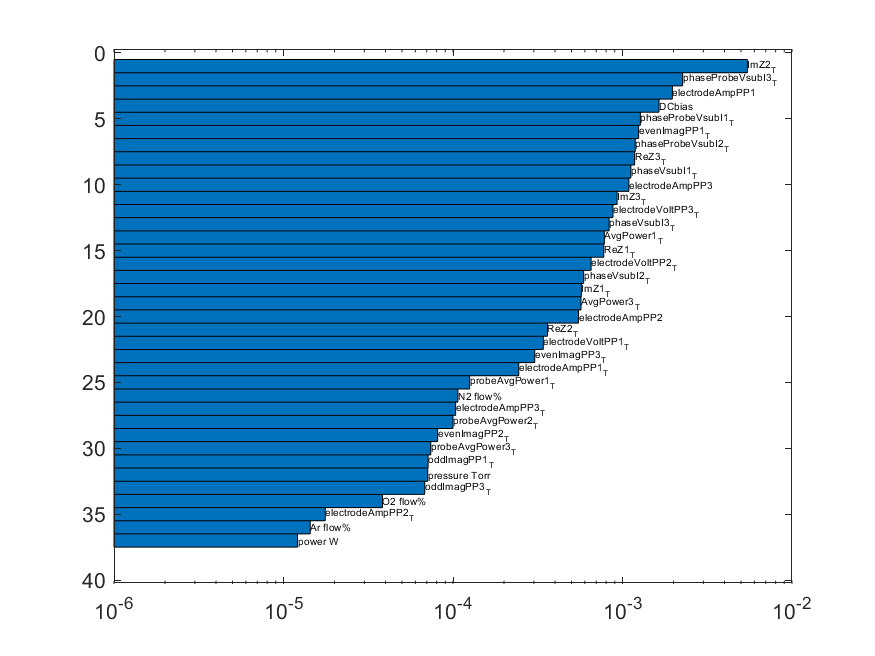
\includegraphics[width=1\textwidth]{input-importance-curvature-testGap.png}
\end{minipage}
\begin{minipage}{0.5\textwidth}
    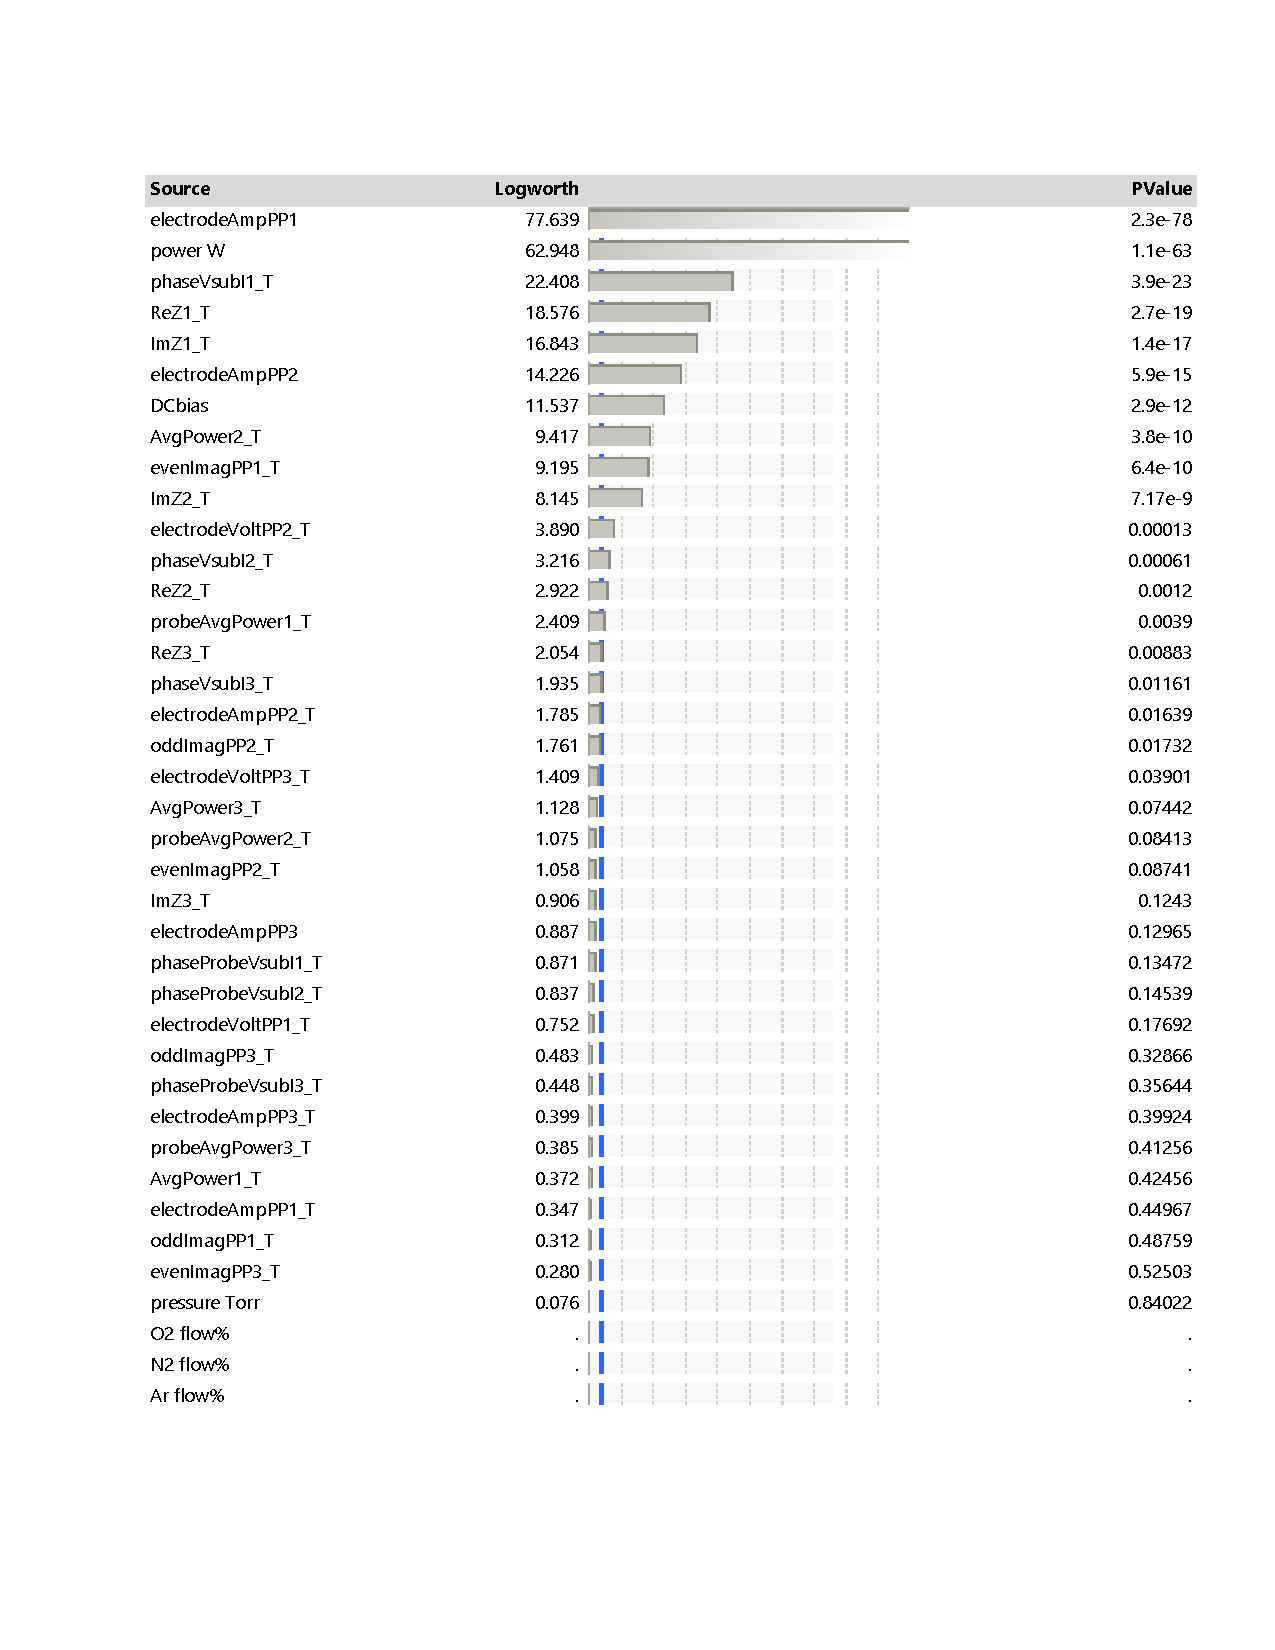
\includegraphics[width=1\textwidth]{jmpGap.pdf}
\end{minipage}

\caption{Predictor importance ranking for electrode gap by random forest (top),  p-value ranking of input parameters for least square fitting electrode gap  (bottom) } 

\label{Fig:gap_SV,pressure_TB,species_TB}
\end{center}
\end{figure}


\begin{figure}[ht!]
\begin{center}
\begin{minipage}{0.5\textwidth}
    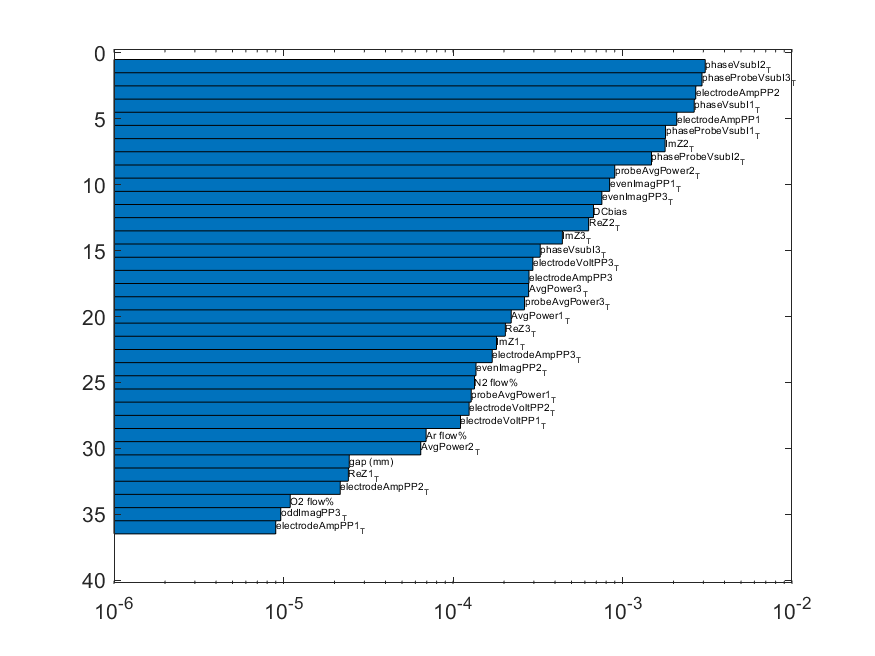
\includegraphics[width=1\textwidth]{input-importance-curvature-testPressure.png}
\end{minipage}
\begin{minipage}{0.5\textwidth}
    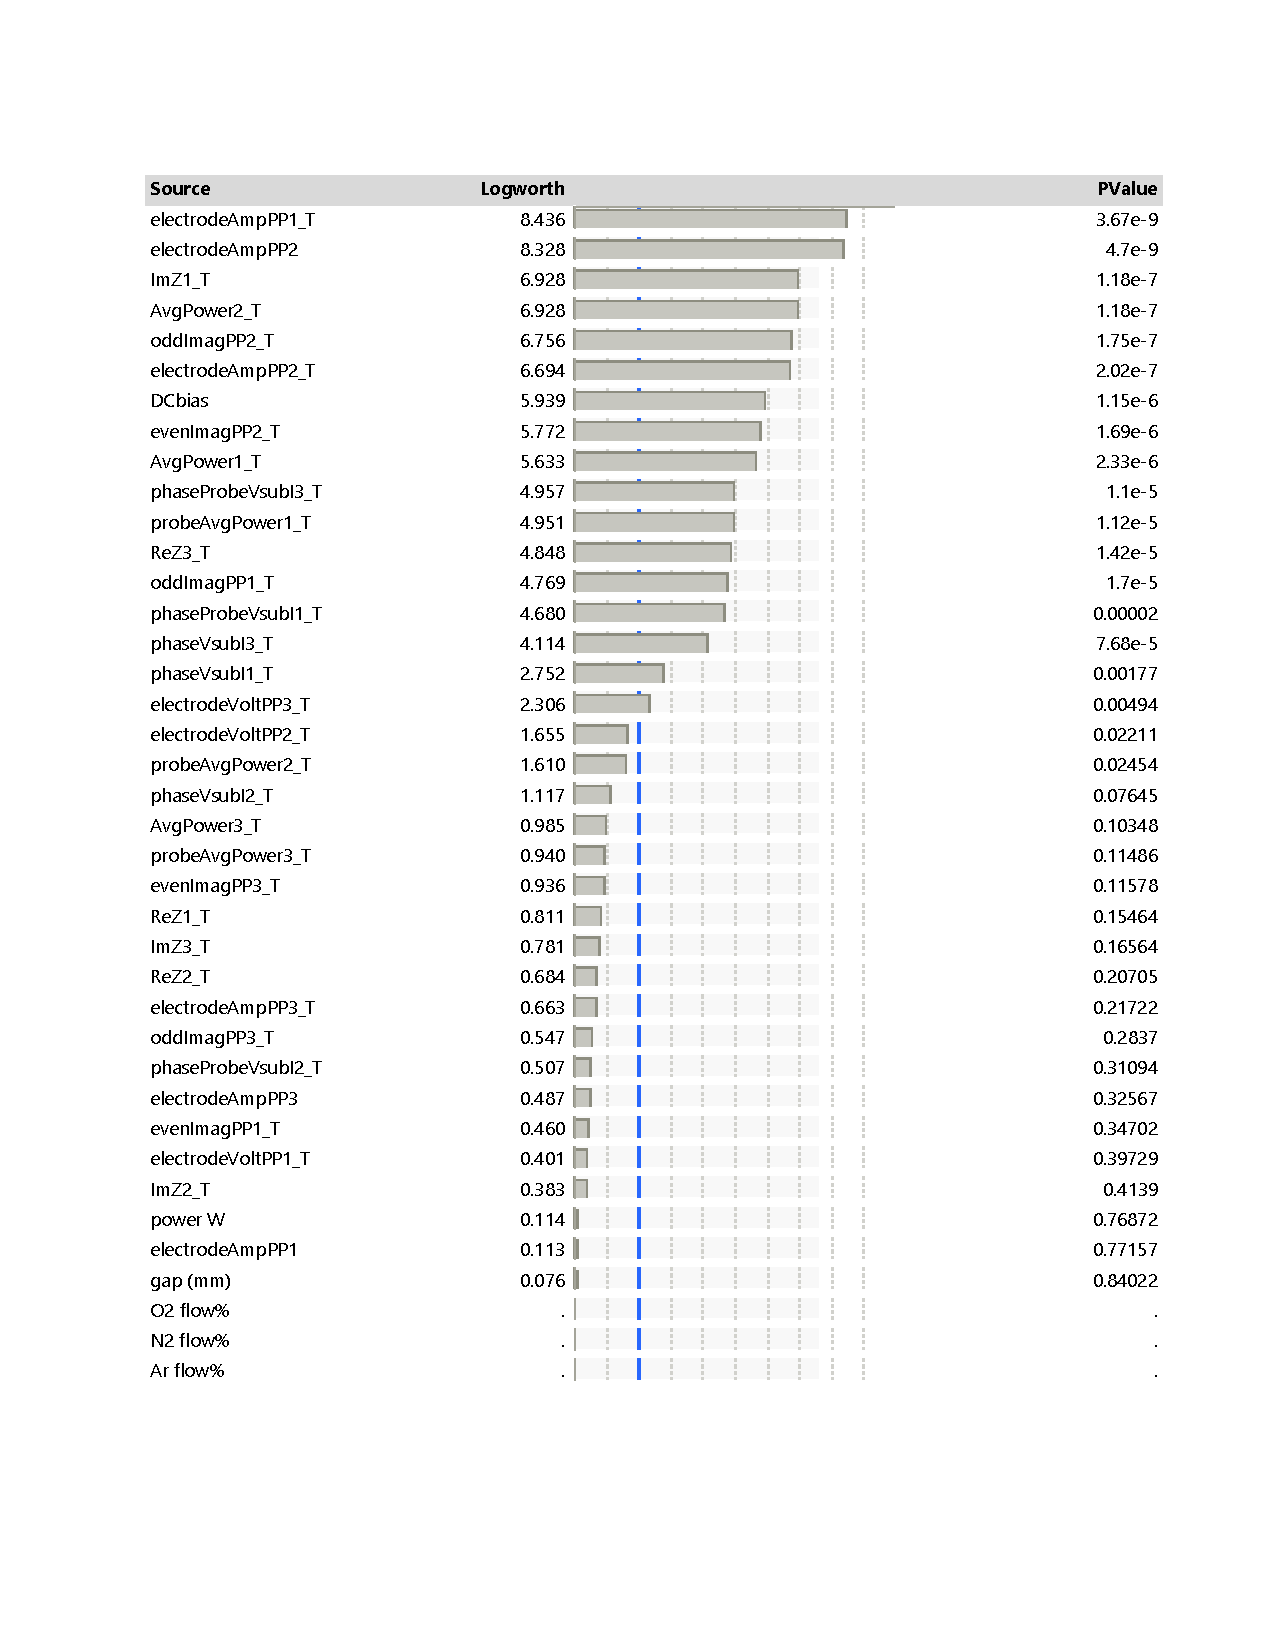
\includegraphics[width=1\textwidth]{jmpPressure.pdf}
\end{minipage}

\caption{Predictor importance ranking for pressure by random forest (top), p-value ranking of input parameters for least square fitting pressure (bottom) } 

\label{Fig:gap_SV,pressure_TB,species_TB}
\end{center}
\end{figure}
Five different classification models were used for comparison for the supervised classification studies namely 1) a neural network model for pattern recognition (patternnet), 2) an ensemble tree model (fitcensemble), 3) a naïve bayes model (fitcnb), 4) a support vector model (fitcsvm) and, 5) a linear discriminant analysis (fitcdscr). These models were used to classify the data by three of the four control parameters namely the operating pressure, gap, and the gas content of the plasma. For classification studies, Matrix 3 was used to check prediction accuracy for a given control parameter using all 34 parameters as well as the remaining control parameters as inputs. The models were randomly trained on 80\% of all 894 observations and tested on the rest 20\% of the observations. The models were optimized during the training. The neural network model was optimized by cross-validating 15\% of the data and testing 15\% of the data while the rest was used for training. The number of hidden layers was 30. On the other hand, the shallow models were optimized by 'automatic' tuning of various parameters that control the learning process i.e the hyperparameters [reference] of the respective models. Moreover, predictors were ranked based on their relative importance using the "out of bag delta error" object under the ensemble tree model. For a given control parameter, a least square fitting optimization was also done with JMP using all remaining parameters as predictors [refer to variable list]. Predictor parameters were ranked in descending order of their p-values. The predictor importance ranking of the random forest model was compared to the p-value ranking for the combined least square fit for the respective control parameter with JMP. \textbf{write comparative analysis of the two rankings}

Both ML and JMP predictions yielded great accuracy [ref. figure]. The p-values between the predictions obtained by a least-square fit and actual values were less than 0.0001 for each classification [refer to table]. On the other hand, all ML models were able to predict the class accurately almost all the time. The Area Under Curve (AUC) [ref] of the Receiver Operating Characteristics (ROC) plots [ref] for each value of all the control parameters was very close to 1. "AUC is the probability that a classifier will be more confident that a randomly chosen positive example is actually positive than that a randomly chosen negative example is positive." Moreover, the effect of principal component analysis (PCA) was also studied for all the classification models. For the PCA studies, components with 99\% cumulative variances were kept. The application of PCA decreased the prediction accuracy substantially. This could be due to the nonlinearity of the I-V dataset.

\textbf{report AUC values as a table and copy confusion matrices from MATLAB for only the best model. Describe the name of the best performing model in text. define AUC in text. Make another table with p-value and correct percent accuracy side by side?}

\begin{figure}[ht!]
\begin{center}
\begin{minipage}{0.495\textwidth}
    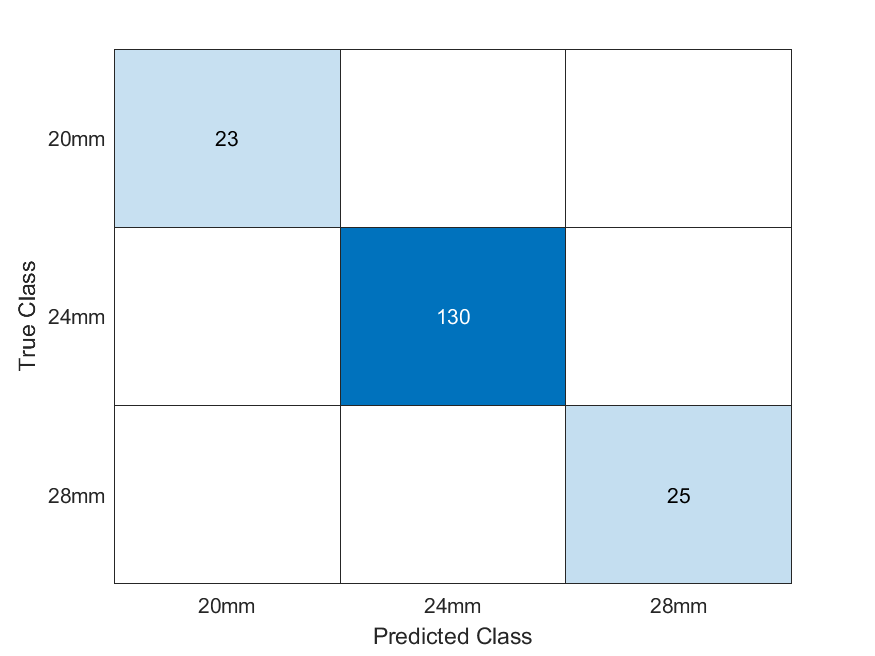
\includegraphics[width=1\textwidth]{ConfusionMatrix_SV.png}
\end{minipage}
\begin{minipage}{0.495\textwidth}
    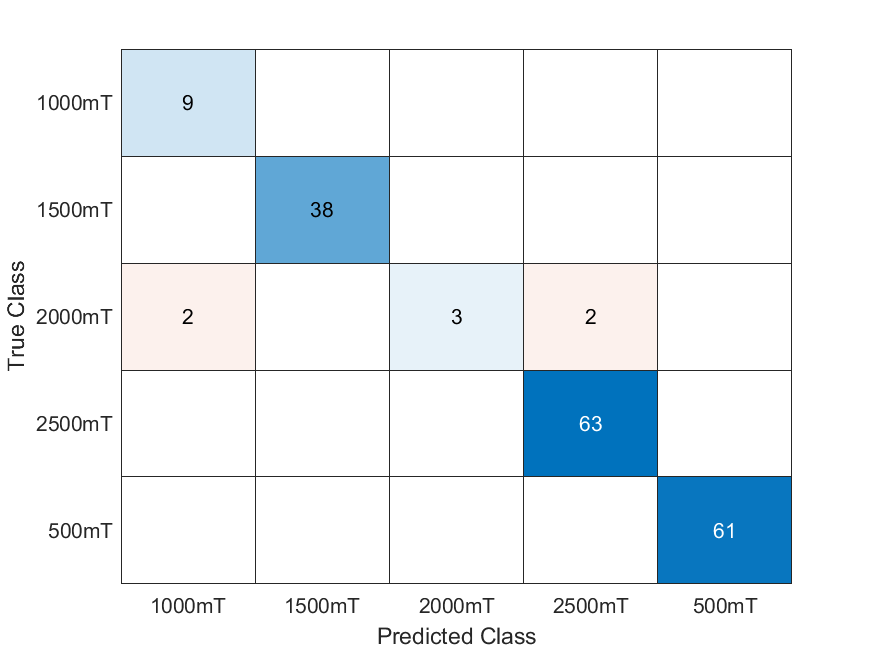
\includegraphics[width=1\textwidth]{ConfusionMatrixTB.png}
\end{minipage}

 \begin{minipage}{0.495\textwidth}
    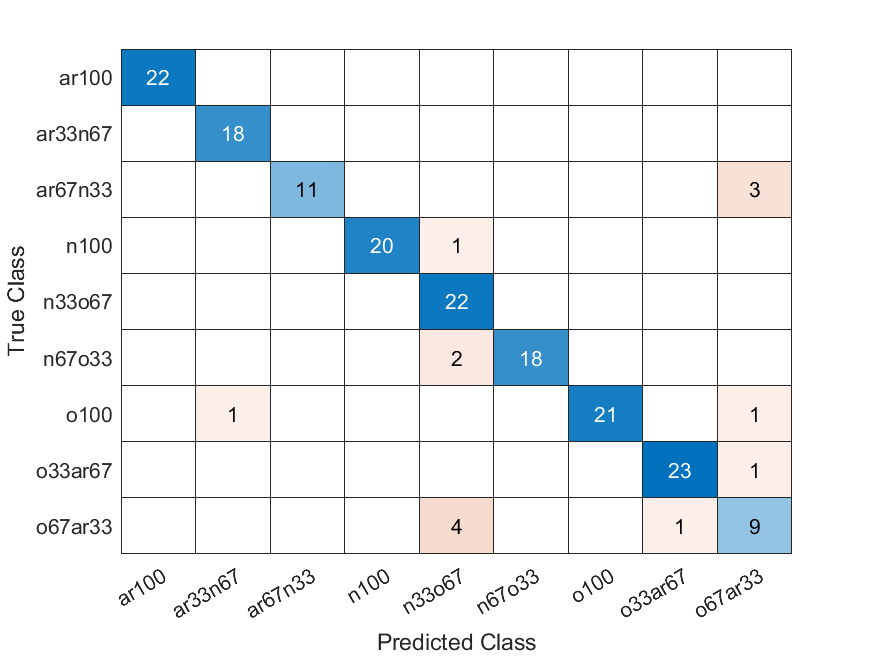
\includegraphics[width=1\textwidth]{ConfusionMatrixTB2.png}
\end{minipage}
\caption{Confusion matrix for Gap (SV) (top left), pressure (TB) (top right), and species (TB) (bottom) } 

\label{Fig:gap_SV,pressure_TB,species_TB}
\end{center}
\end{figure}


\section{Conclusions and future work}\label{Sect:Conclusions}

In this article, we have used statistical as well as machine learning predictions to analyze and organize I-V data in a moderate pressure capacively coupled plasma (CCP). We have demonstrated that deep neural network (DNN) as well as shallow machine learning models can be a useful tool for extrapolating data even with a high error bar at a transitional regime. Specifically, phase data with high error bars can be predicted with great accuracy which can be used to automatically tune matching networks. Classification of control parameters is another possible application of these models given a large set of measured data is available. The models were able to identify the gas ratio in the feed gas as well as correctly identify the operating pressure and electrode gap in almost all the cases. The importance of the predictors was ranked for these classification predictions. While input parameter importance can give some insight into the physics, comparison with physics-informed models is necessary. In future works, Physics-informed learning, such as physics-informed neural networks (PINNs) [ref-nature paper] will be explored on the mGEC moderate pressure database. Physics-informed learnings, can integrate domain knowledge and physical laws into ML models, improving their interpretability and accuracy, even with imperfect data. The availability of data and complexity of the system influence the specific data-driven approach for predictive modelling.



\section{Acknowledgements}
This work was supported by a generous donation from Applied Materials Inc.

\printbibliography %Prints bibliography


\end{document}

